\documentclass{report}
\usepackage[norsk]{babel}
\usepackage[margin=6pc]{geometry}
\usepackage{graphicx}
\usepackage{float}
\usepackage[hidelinks]{hyperref}
\usepackage{amsmath}
\usepackage{float}
\DeclareUnicodeCharacter{2212}{-}


\begin{document}
\date{\today}
\begin{titlepage}
	\centering
	\vfill
	{\bfseries
		\Huge Torsk I Barentshavet\\ \Large
		Analysere utviklinga av Atlantisk Torsk i Barentshavet.\\
		\vskip2cm
		Are Olsen, 2STA, Vardafjell vgs.\\
		7600 Ord. 24.03.2023.
	}
	\vfill
	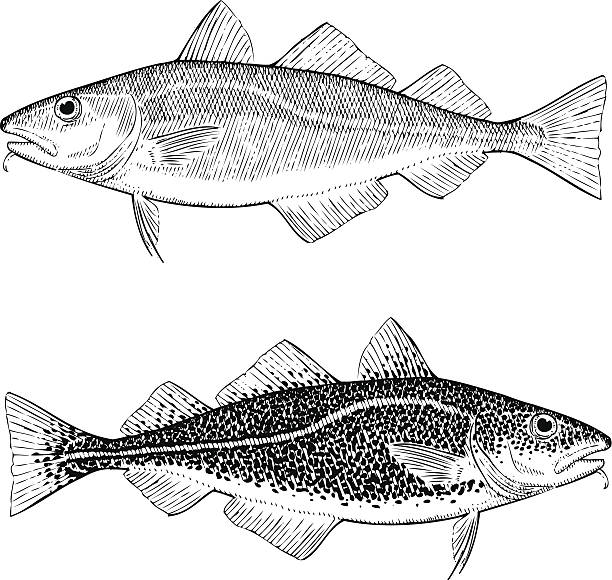
\includegraphics[width=9cm]{Bileter/Torsk.jpg} % also works with logo.pdf
	\vfill
	\vfill
\end{titlepage}



\tableofcontents

\chapter{Introduksjon.}
Dette matematikkprosjektet i faget R1 er ein ambisiøs satsing som tek sikte på å gjennomføre ein grundig analyse av ulike datasett, samt å utføre ein omfattande matematisk undersøking av dei aktuelle dataene. Prosjektet vil ha ei varigheit på to veker, der fem skuletimar vil vere tilgjengeleg per veke, med ein total tidsramme på ti skuletimar.
Mitt val av tema for prosjektet er å analysere ein fiskebestand, og eg ynskjer å undersøke ulike faktorar som kan påverke bestanden. Dette vil vere en krevende oppgåve, og eg har valgt å bruke mine matematiske ferdigheiter til å undersøke og analysere korrelasjoner mellom ulike faktorar og fiskebestanden. Med denne tilnærmingen håper eg å kunne skaffe ein dypere innsikt i kompleksiteten som omgir fiskebestandar, og kanskje til og med bidra til å finne måter å forbedre forvaltningen av slike ressursar på.
Eg ser fram til å utforske denne tematikken nærmere, og eg er ivrig etter å ta i bruk mine ferdigheter i matematikk til å analysere dette interessante datasettet. Med grundige analyser og presis matematisk modellering håper eg å kunne bidra til en bedre forståelse av fiskebestanden og dens påvirkningsfaktorer.
\section{Emnet og problemstillinga.}
Den utvalde fiskebestanden for mitt prosjekt er \textit{atlantisk torsk} som befinner seg i Barentshavet i ``ICES SUBAREA 1``.
Hovedproblemstillinga i prosjektet mitt er å analysere korleis fiskebestanden av torsk vil utvikle seg, skape matematiske modellar som gjer det mogleg å modellere torskebestanden med hovudsakeleg omsyn til tid, og forsøke å gjere det same med andre miljø faktorar som temperatur og salinitet.
Ikkje minst, undersøke korleis bestanden veks og minkar, når den er på det høgaste og det lågaste, et cetera.
Vidare ynskjer eg å forsøke å anslå kva torskebestanden kan omtrentleg vere, og eventuellt anslå kor presis modellane framstilt er.
Målet med prosjektet er å utvikle matematiske modellar og kunnskap rundt denne fiskebestanden slik at den kan bli brukt for ein berekraftig forvalting av fiskebestanden i post-oljetida i Noreg.
\section{Hypoteser.}
Hypotesen som blir presentert, hevder at torskebestanden vil bli påverka av ulike faktorar, særleg miljømessige faktorar og endringar i miljøet, samt av andre fiskebestandar som både fungerer som rovdyr og bytte. Det er hevda at endringar i desse bestandane vil ha ein direkte innverknad på torskebestanden, og at ein auke eller reduksjon i desse bestandane vil ha ei tilsvarende effekt på torskebestanden.
Framover i tid vil torskebestanden truleg halde seg meir eller mindre konstant, sidan andre fiskebestandar kan leve i ein form for samspel der dei held seg i sesongar, og miljøfaktorar kan moglegvis ha ei minimal og ubetydeleg effekt. Dette betyr at torskebestanden vil trulegvis halde seg på eit relativt stabilt nivå i framtida.
Det er likevel verdt å merke seg at eventuelle anomalier eller avvik frå denne trenden kan moglegvis bli forklart gjennom fiskesesongar og menneskeleg innverknad. Dette kan vere viktige faktorar som kan påverke torskebestanden på kort og lang sikt.
I lys av desse faktorane kan det hevdast at torskebestanden vil halde seg relativt stabil, men at den likevel kan vere påverka av ulike faktorar som miljø og menneskeleg aktivitet.
\section{Relevanse.}
Fiskebestanden av torsk i Barentshavet er av betydeleg interesse for meg av ein rekke grunnar. Sjølv om bestanden ikkje har ein direkte påverknad på meg som individ, er eg likevel opptatt av fiskeri og fiskeindustrien, som kan komme til å utgjere ein viktig del av Noregs økonomi i post-oljetida.
I tillegg er eg svært interessert i politikk, og debattar rundt fiskeindustrien har vore eit tilbakevendande tema i den norske politiske arenaen. Spørsmål som om Noreg skal bli med i EU, har potensiale til å påverke fiskebestanden og fiskeriindustrien på ein direkte måte. Dermed er eg motivert for å følgje med på utviklinga i fiskeripolitikken.
Det er heva at torsk i Barentshavet kan vere ein viktig faktor i Noregs framtid, og det er dermed relevant for meg å halde meg oppdatert på utviklinga i denne sektoren. Eg føler at dette er relevant for meg på grunn av min interesse for fiskeri, politikk og den potensielle påverknaden det kan ha på landet vårt i framtida.
Med omsyn til dei ovan nemnde faktorane kan det konkluderast med at fiskebestanden av torsk i Barentshavet er av stor interesse og relevans for meg som ein engasjert borgar og eit potensielt medlem av arbeidsstyrken i framtida. Det er derfor viktig å vere medvitne om utviklinga i denne sektoren for å kunne gjere informerte og strategiske avgjerder i framtida.

\chapter{Teori.}
\section{Biologi Teori.}
\subsection{Miljø påverknader til fiskebestander.}
Fiskebestandar er avhengige av fleire miljøfaktorar for å trivast og oppretthalde ein sunn bestand. Desse faktorane varierer stort avhengig av art og habitatet fisken lever i. Temperatur og salinitet er eksempel på faktorar som ofte vert sterkt tilknytt til ein fiskebestands helse og overleving.
Temperatur er rekna som ein av dei viktigaste miljøfaktorane som påverkar fiskebestandar, og forsking har vist at sjølv små endringar i vanntemperaturen kan ha ein betydeleg innverknad på både vekst, overleving og reproduksjon. Det finst fleire måtar temperatur kan påverke fiskebestanden på. Til dømes kan høgare vanntemperaturar auke fisken sin metabolisme og behov for mat. Dersom dette ikkje blir kompensert ved ein tilsvarande auka tilgang på mat, kan det føre til underernæring og svekka overleving. Vidare kan høge temperaturar også føre til oksygenmangel i vatnet, som igjen kan føre til kvelning og død blant fiskebestanden.
Salinitet er ein annan viktig faktor som påverkar fiskebestandar. Salinitet refererer til mengda salt i vatnet, og kan variere betydeleg avhengig av geografisk plassering og tidevatnsforhold. Fisk som lever i saltvatnsmiljø, slik som laks og torsk, er avhengige av ein vis salinitet for å trivast. For høge eller for låge salinitetsnivå kan føre til stress og svekka helse.
Det finst også andre miljøfaktorar som kan påverke fiskebestandar, inkludert pH-nivå, tilgang på mat og tilstedeværelsen av sjukdommar og parasittar. Sjølv om det finst ein generell tilknyting mellom ulike miljøfaktorar og fiskebestandar, kan verknaden av desse faktorane variere stort avhengig av art og habitat. Til dømes kan ei viss temperatur som fungerer optimalt for éin art, ha ein negativ innverknad på ein annan.
Det er difor viktig å forstå korleis ulike miljøfaktorar kan påverke fiskebestandar, og korleis ein kan tilpasse seg endringar i miljøet for å beskytte fiskebestandane på lang sikt. Vidare forsking og observasjonar vil bidra til å utvide vår kunnskap om korleis ulike faktorar samspelar for å påverke fiskebestandar, og korleis vi kan ta ansvarlege avgjerder for å beskytte desse økosystema.
(Wikipedia, 2023).
\subsection{Samspel mellom ulike fiskebestander.}
Fiskebestandar er ein sentral del av økosystemet i havet, og ulike fiskearter kan ha ei direkte eller indirekte innverknad på kvarandre gjennom næringskjeden. Næringskjeden i havet er kompleks og dynamisk, og ulike fiskearter kan vere direkte tilknytt til kvarandre gjennom mat og beite, men også gjennom andre faktorar.
Eit døme på direkte tilknyting gjennom næringskjeden er når ein fiskeart spis ein anna.
Dersom ein predatorfisk reduserer talet på ein byttefisk kan dette føre til mangel på mat for andre predatorfisk som er avhengige av same byttefisk. Dette kan igjen påverke bestanden av andre fiskearter som deler same økosystem.
Ein slik direkte tilknyting kan ofte oppstå når fleire fiskearter er avhengige av same byttefisk.
Indirekte tilknyting mellom fiskearter kan vere meir kompleks. Dette kan skje gjennom for eksempel utvikling av konkurranse om ressursar, eller gjennom samarbeid og gjensidig nytte. Ein fiskeart som utkonkurrerer ein anna fiskeart om mat eller beite, kan påverke den andre fiskearten gjennom reduksjon av mat eller nedgang i vekst. På den andre sida kan samarbeid mellom fiskearter gjennom samliv og symbiose, føre til ein positiv effekt på bestanden. Eit døme på dette kan vere når reker eller krill renser parasittar frå huda til andre fiskearter.
Til tross for at fiskeartar kan ha komplekse tilknytingar til kvarandre, kan desse tilknytingane også variere i stor grad over tid. Dette kan skje gjennom sesongmessige variasjonar, for eksempel når ulike fiskebestandar migrerer til andre område for beite eller gyting. Ein endring i ein fiskebestand kan også føre til endringar i andre fiskearter som er avhengige av same økosystem.
Å forstå samspela mellom ulike fiskebestandar og korleis dei påverkar kvarandre er avgjerande for å oppretthalde ein sunn og bærekraftig fiskeindustri. Dette inneber å studere næringskjeden og økosystemet i havet for å identifisere kritiske faktorar som kan påverke bestandane. Det kan også innebere å ta ansvarlege avgjerder for å sikre at fiskebestandane blir forvalta på ein bærekraftig måte.
(Wikpedia, 2023.)
\chapter{Analyse.}
\section{Forandring av datasett.}
I denne undersøkinga har det vore utfordrande å jobbe med ulike datasett og innsamlingsmetodar, som har ført til at datasettet har måtte bli korta ned til å berre innehalde data samla inn mellom 1987 og 2014. Dette har vore naudsynt på grunn av ulike start- og slutt-tider på innsamling av data og ulike innsamlingsmetodar, som har gjort det vanskeleg å samle alt data i eitt datasett. Datasettet består av data frå \textit{SJØMIL} under Havforskningsinstituttet, og er avgrensa til \textit{ICES SUBAREA 1} i Barentshavet. Sjølv om det kunne vore ønskeleg å inkludere data utanfor dette tidsområdet, var dette ikkje mogleg ettersom det kunne ha ført til ein mangel på informasjon om eventuelle anomaliar i datasettet.
Dette datasettet fokuserer på fleire variablar, som temperatur og salinitet ved Vardø, ein kommune som ligg langs den nordlege norske kysten i Barentshavet. I tillegg inneheld datasettet informasjon om mengda zooplankton observert per kvadratmeter areal over Barentshavet i \textit{ICES SUBAREA 1}, samt mengden lodde og torsk funne i dette området.
Sjølv om datasettet er kortare enn ønskeleg, er det viktig å merke seg at dette ikkje nødvendigvis betyr at det er dårleg eller av mindre verdi. Tvert imot inneheld datasettet mykje informasjon som kan vere korrelert og relevant for undersøkingane som skal utførast. Denne undersøkinga er ein slags pioner innanfor dette feltet, og den korte tidsperioden som er dekt i datasettet er ein påfølgjande krav til slike nye dataundersøkingar. \\
\\
Etter å ha begrenset datasettet og samlet datasettet til eit, var datasettet ført inn i det matematiske rekneprogrammet \textit{GeoGebra} under \textit{Rekneark}-et slik at datasettet var klar for analyse og eventuelle matematiske undersøkingar.
\begin{figure}[H]
	\centering
	\fbox{
		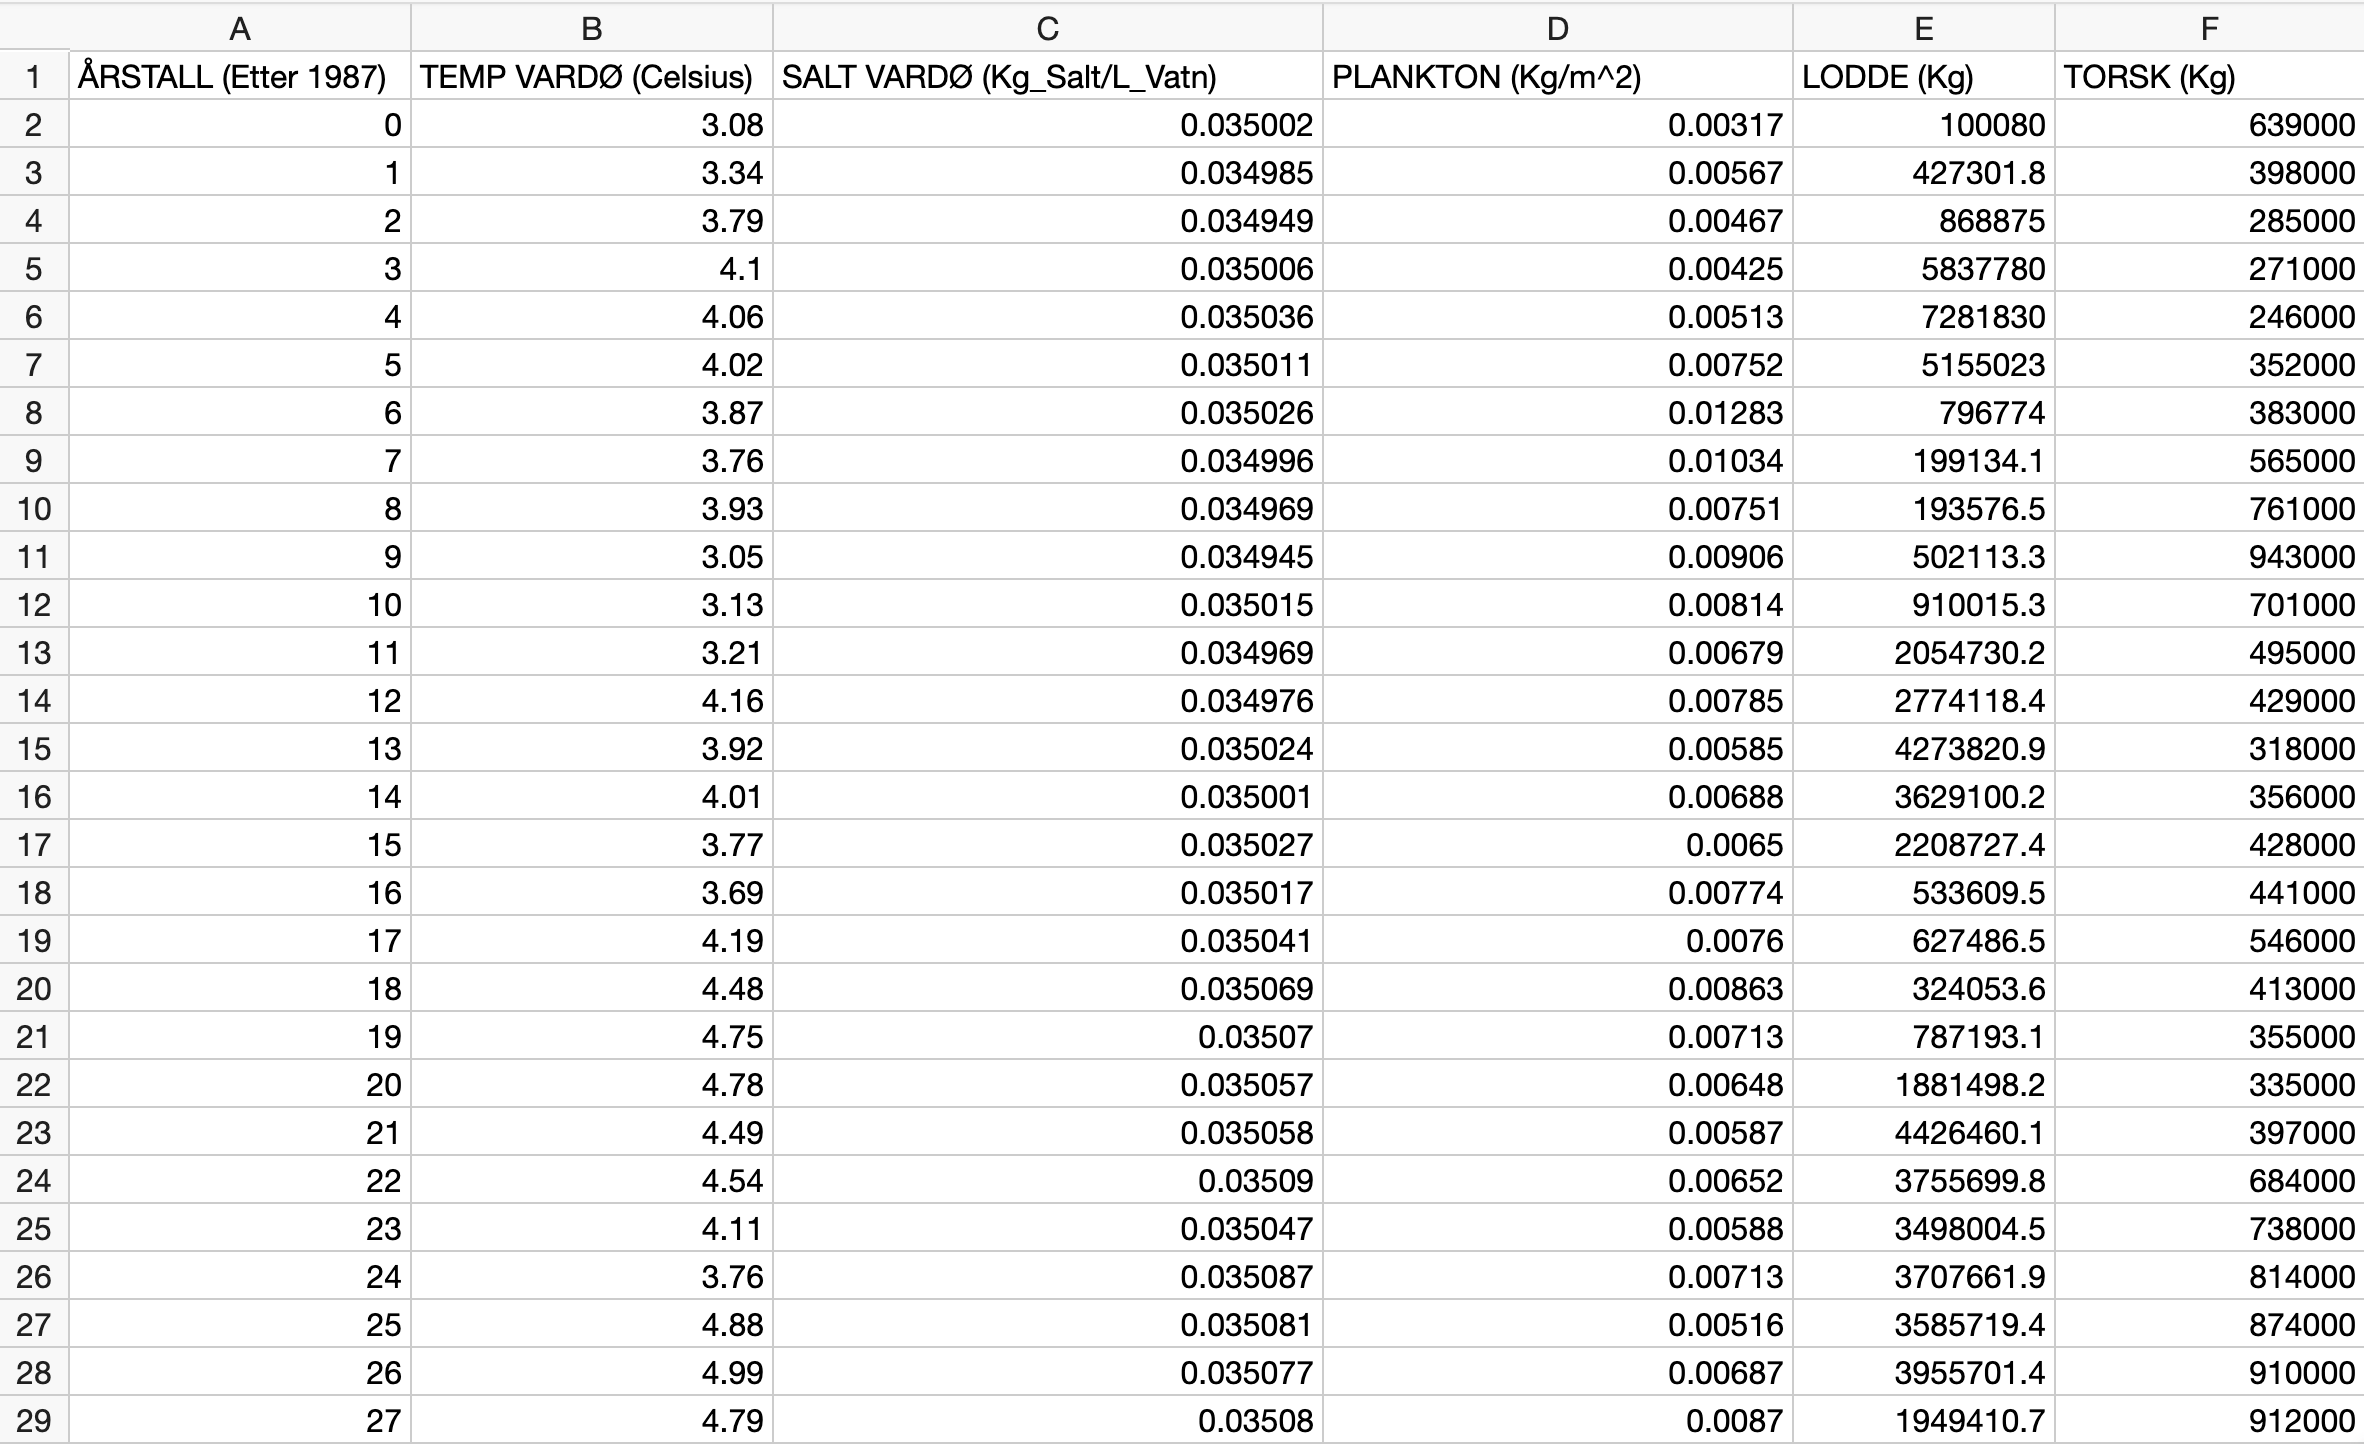
\includegraphics[scale=0.5]{Bileter/Datasettet.png}
	}
	\caption{Datasettet i Geogebra Rekneark.}
	\label{F2}
\end{figure}\newpage
\section{Plotte data.}
Ved å importere datasetta frå det opphavlege regnearket over til det visuelle kartesiske planet, også kjent som grafikk-feltet, gjennom bruk av lister og funksjonen \textit{Polylinje(liste)} i GeoGebra, vart det etablert ein metode for å generere ein meir systematisk og oversiktleg framstilling av dataa. Denne teknikken tillét ein grundigare visualisering og ein meir komplett oversikt over dei tilgjengelege datasetta og deira ulike potensielle variablar.
Denne framgangsmåten i analysen var av særleg betydning for å kunne tilby ein meir omfattande og detaljert visuell representasjon av dataa og deira eventuelle samanhengar. Den tillét òg ein meir inngåande undersøking av ulike relasjonar mellom dei ulike datasetta, for eksempel at loddebestanden sin auking ledet i etterkant til ein auking i torskebestanden, noko som ville vere vanskeleg å oppdage gjennom ein manuell analyse av regnearket.
Ved å ta i bruk denne tilnærminga, kunne det observerast at det var mogleg å identifisere potensielle årsaks-verknadsforhald mellom dei ulike datasetta og deira variablar. Dette ga rom for ein meir omfattande analyse av datasetta og gjorde det mogleg med djupare undersøkingar av samanhengane som eksisterte mellom dei.

\begin{table}[H]
	\centering
	\begin{tabular}{|l|l|l|}
		\hline
		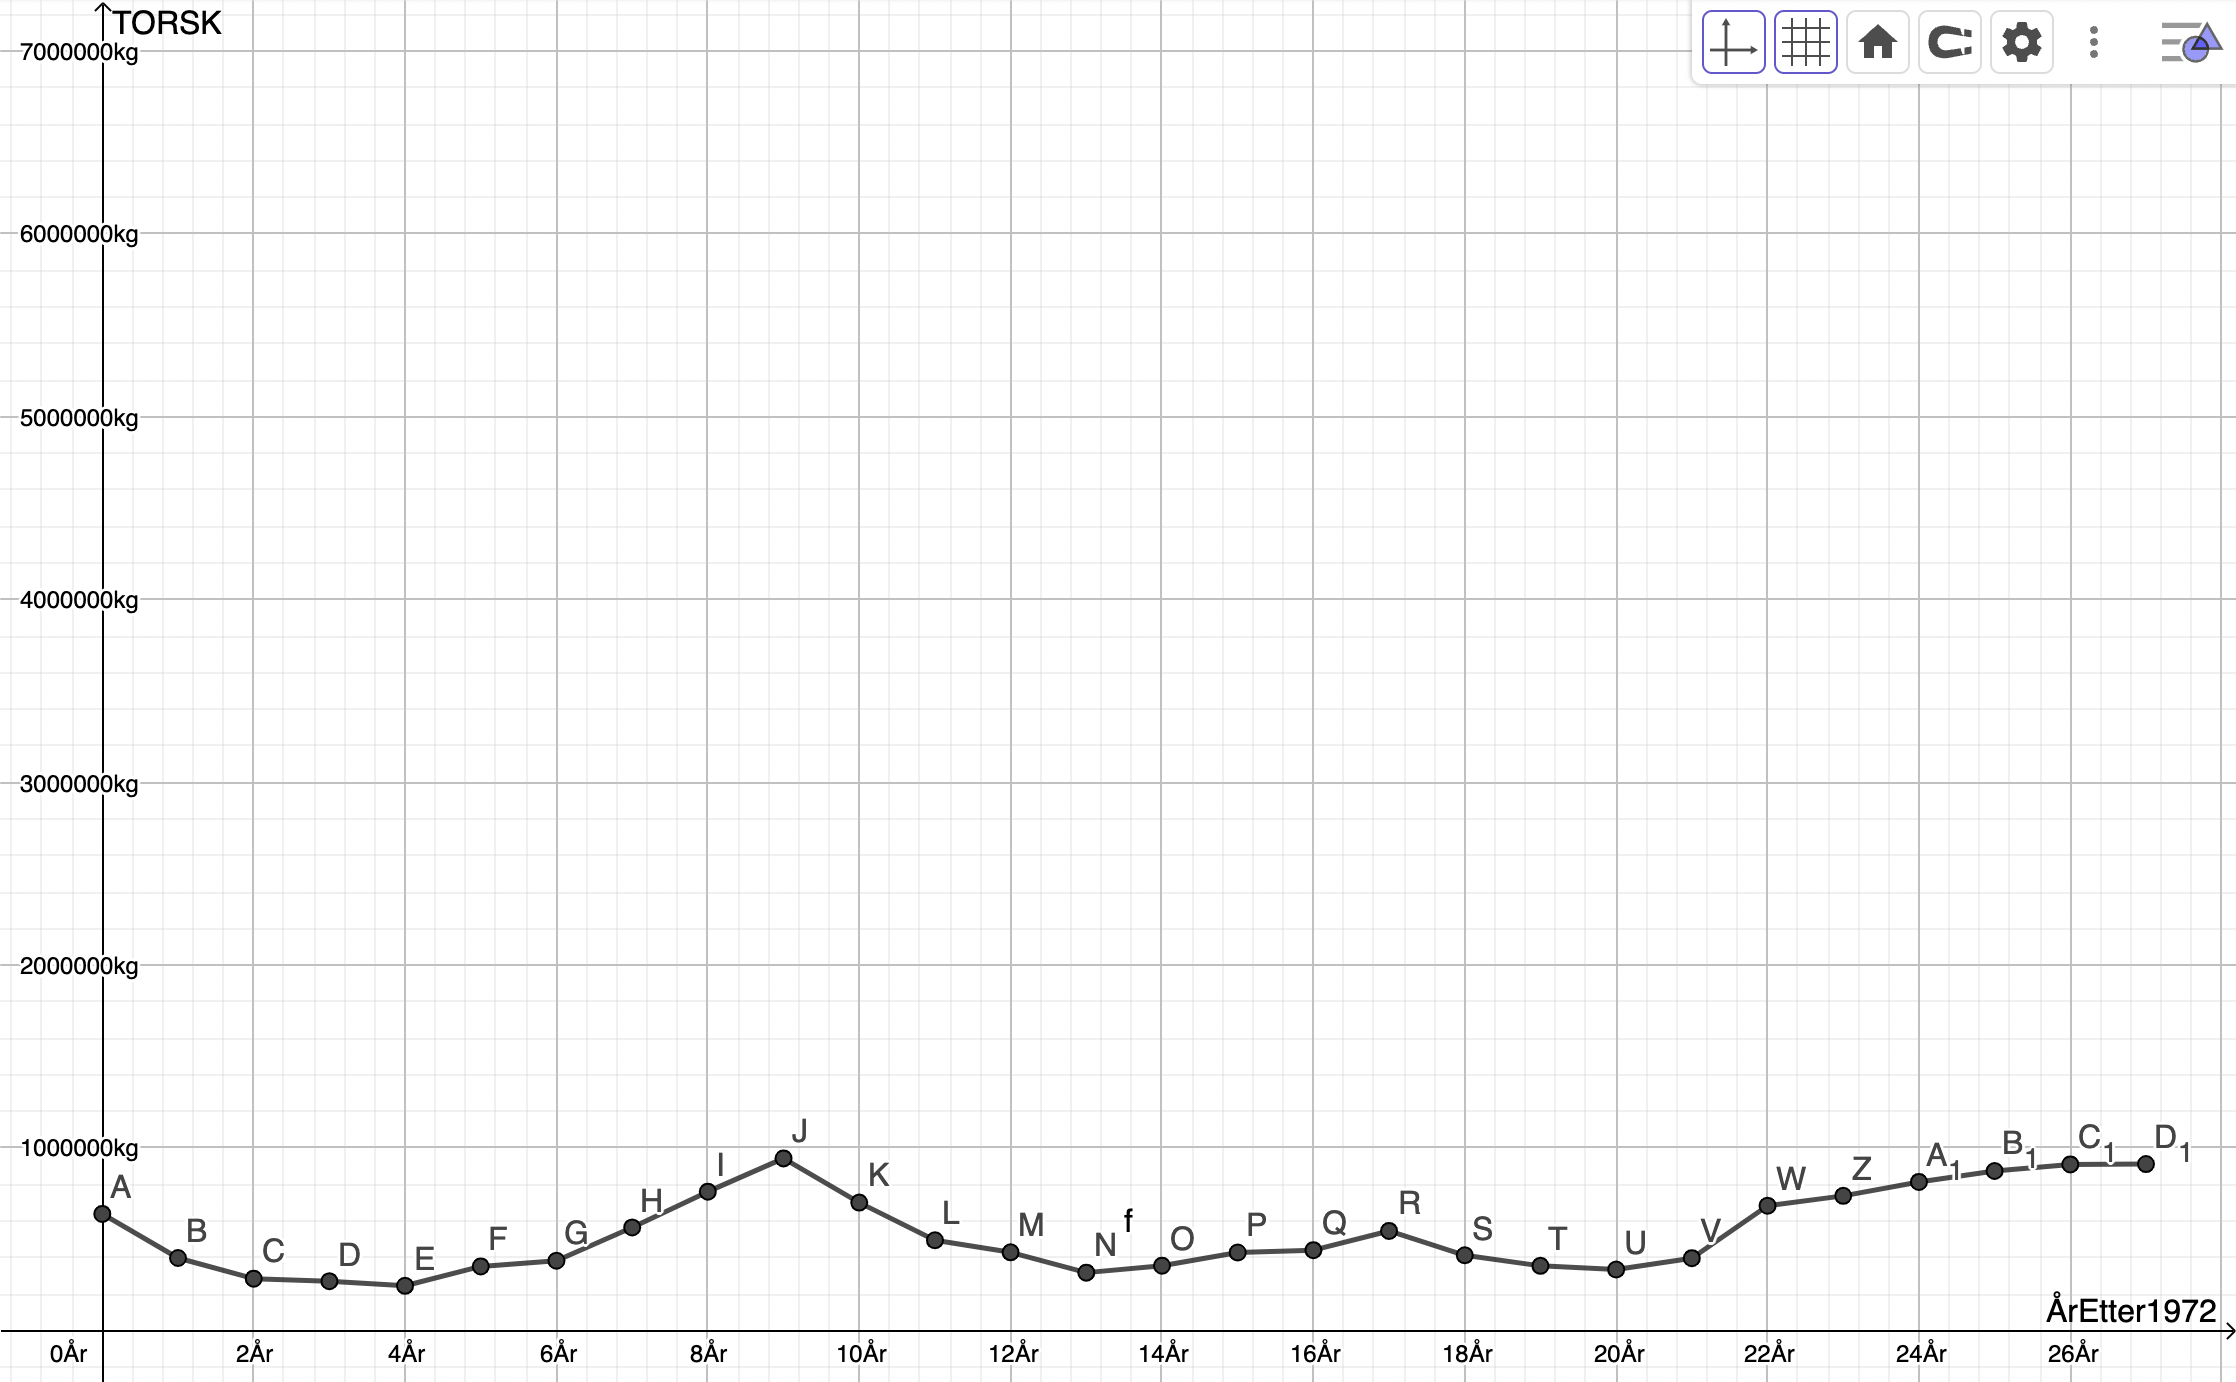
\includegraphics[width=5.5cm]{Bileter/Torsk.png} & 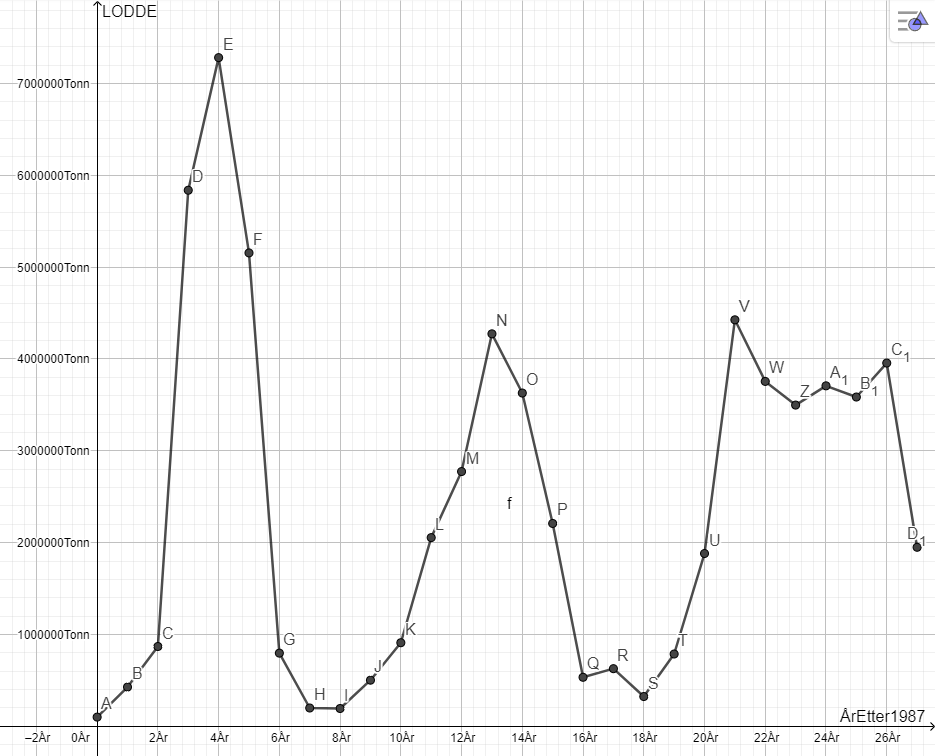
\includegraphics[width=5.5cm]{Bileter/Lodde.png} & 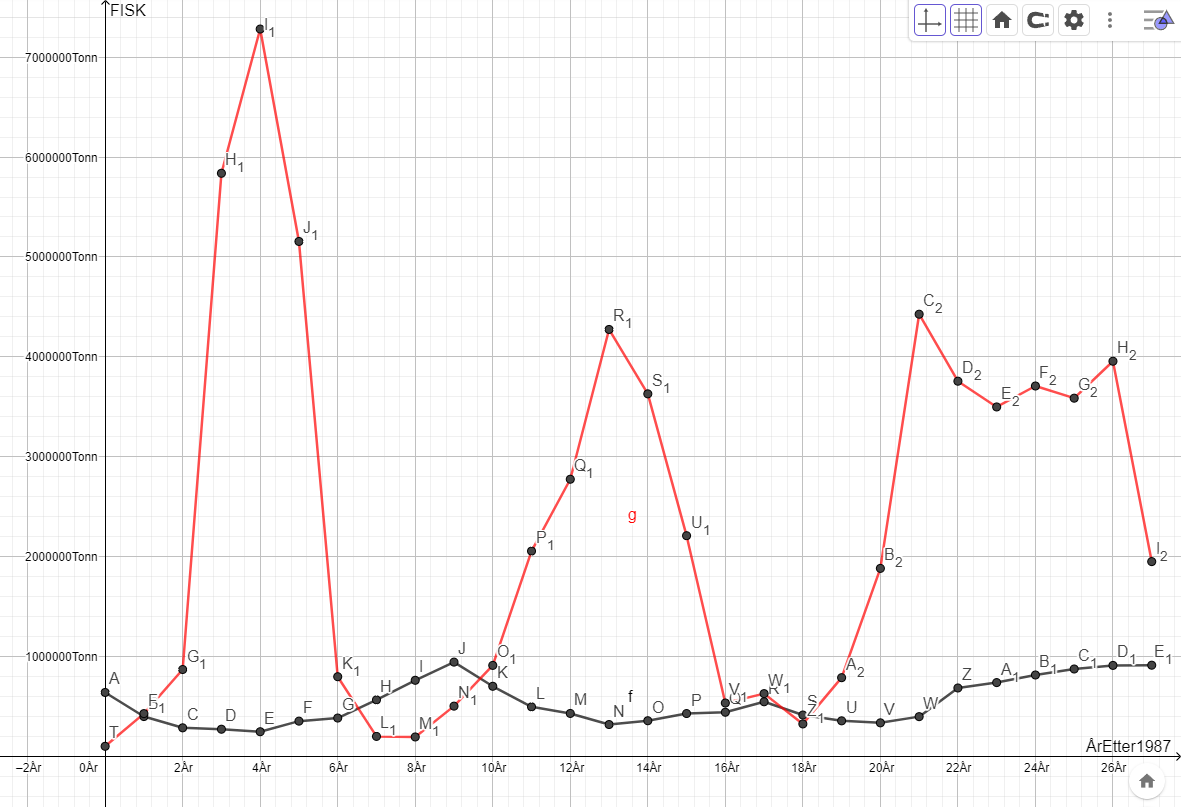
\includegraphics[width=5.5cm]{Bileter/loddeogtorsk.png} \\
		\hline
		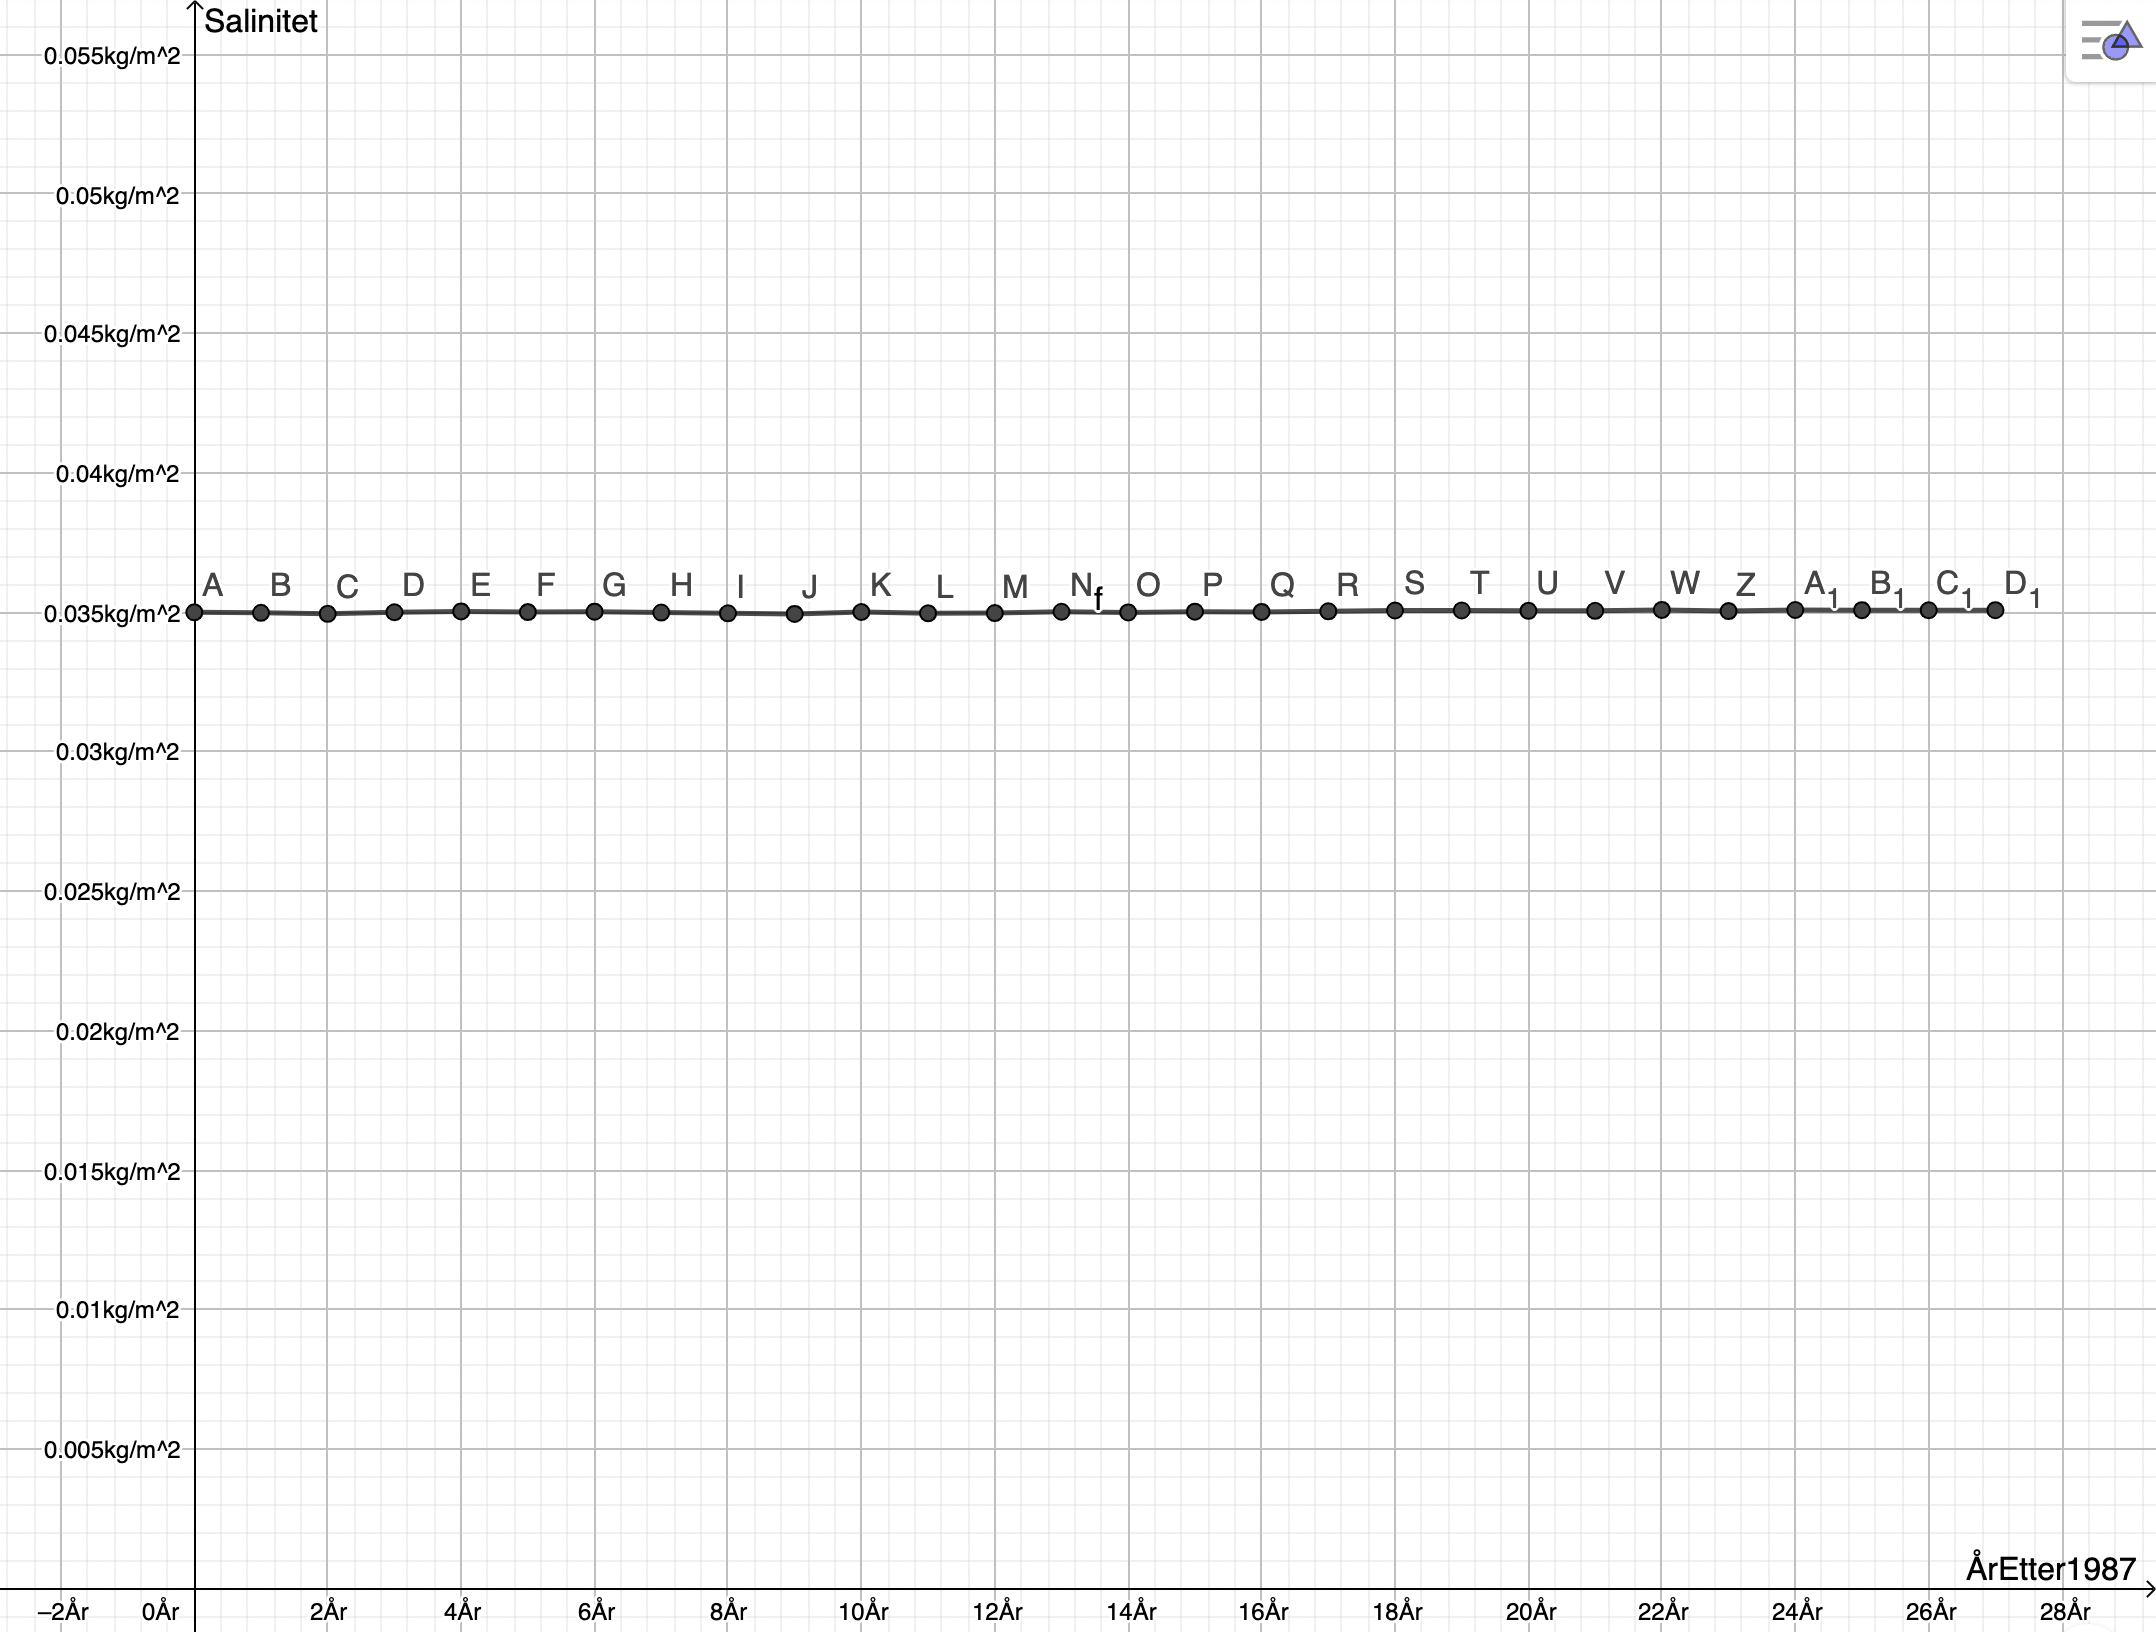
\includegraphics[width=5.5cm]{Bileter/Salt.png}  & 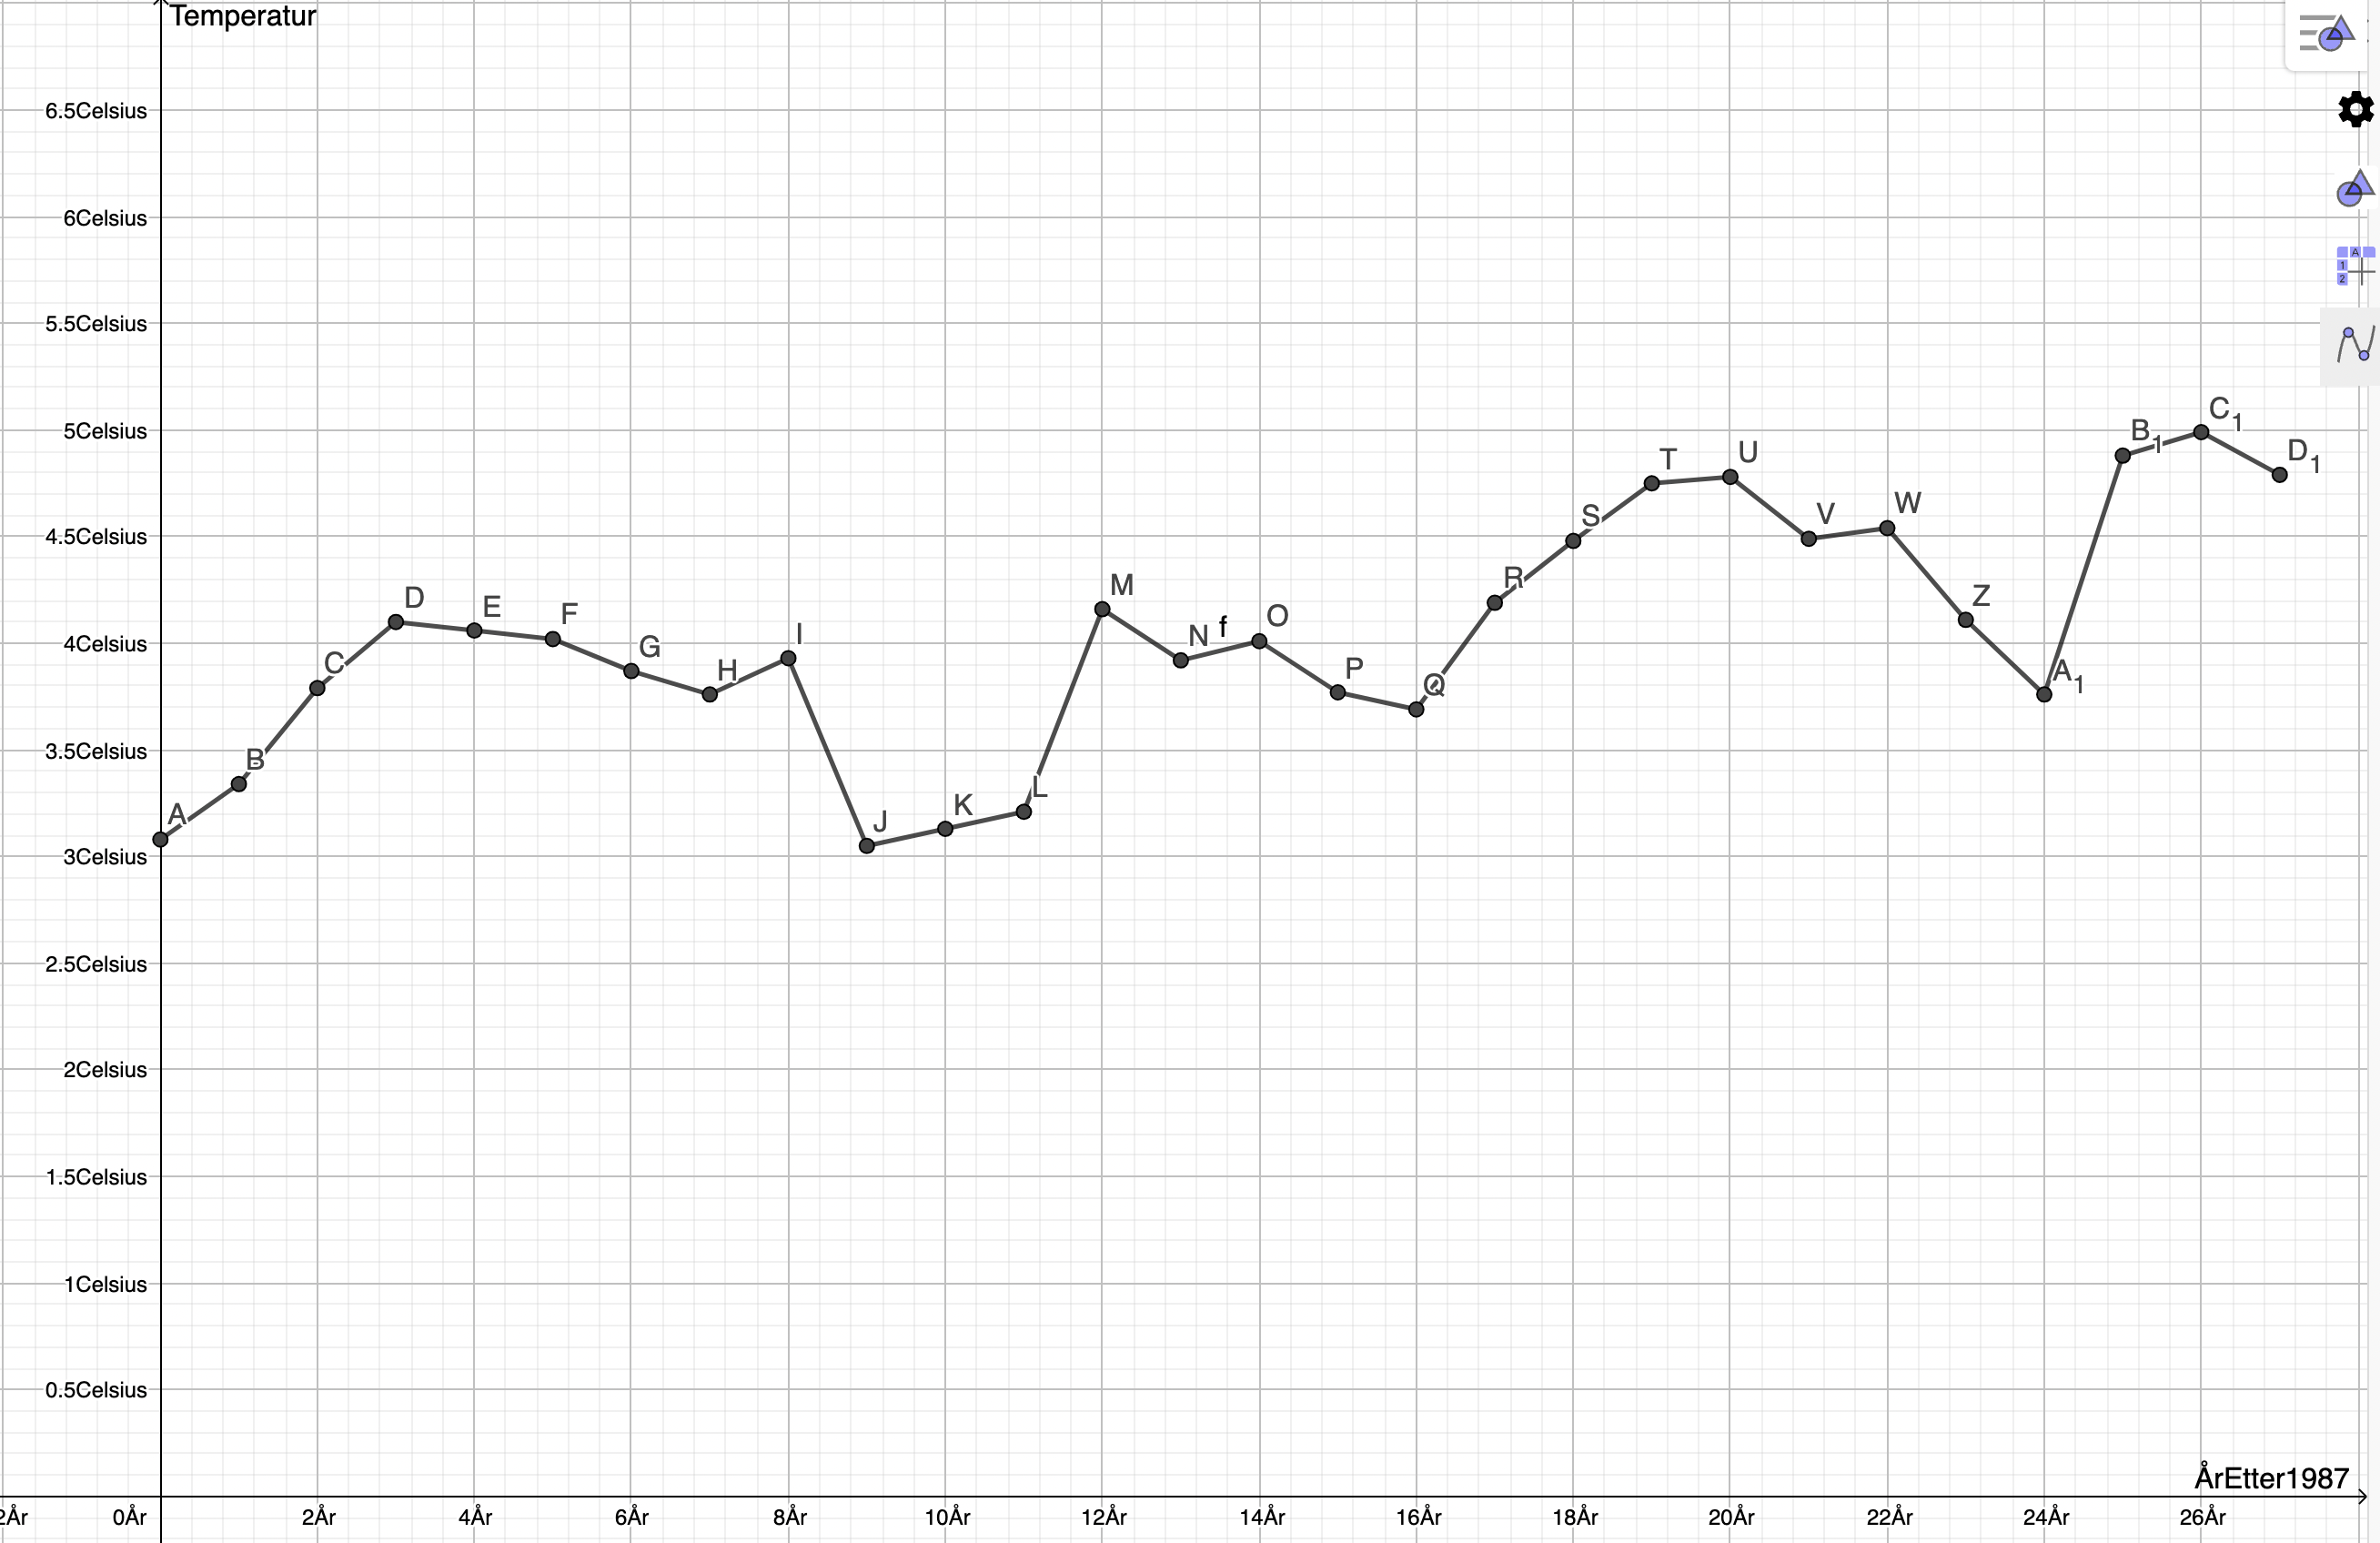
\includegraphics[width=5.5cm]{Bileter/Temp.png}  & 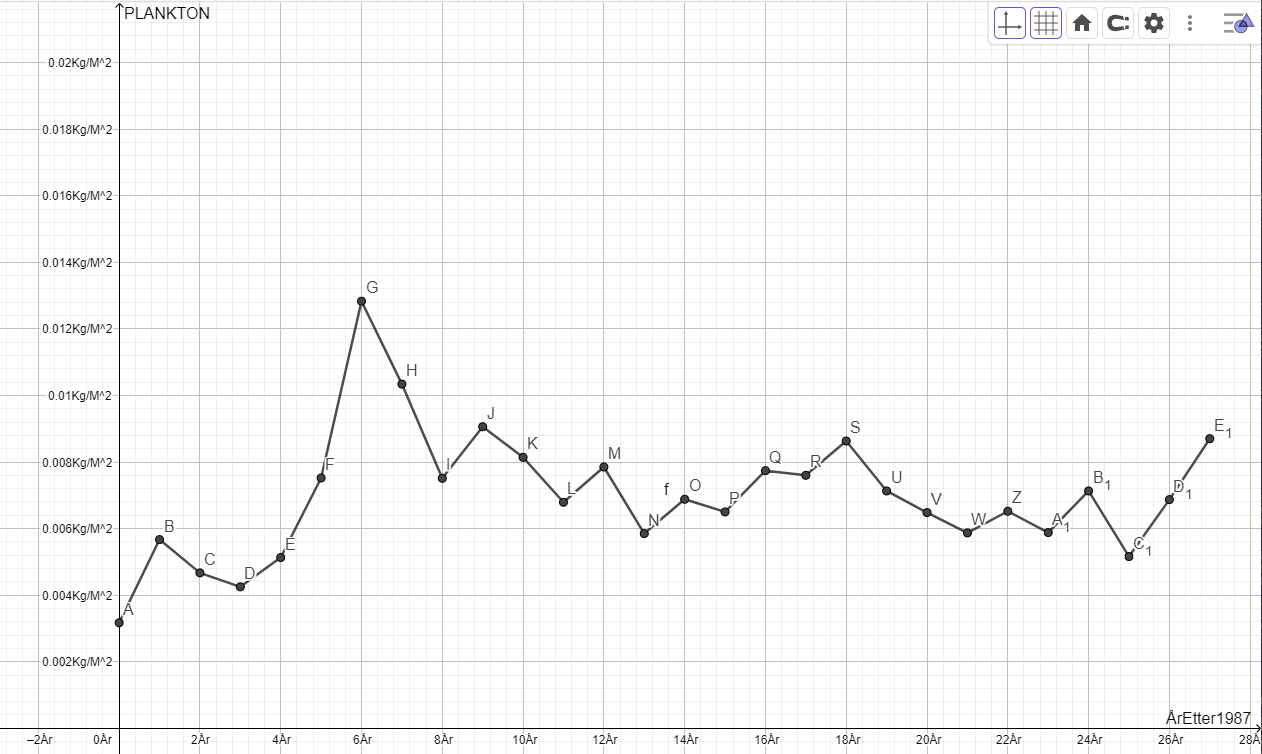
\includegraphics[width=5.5cm]{Bileter/PLANKTON..png}    \\
		\hline
	\end{tabular}
	\caption{Alle dataplottingane i det kartetiske planet. (Graf har datasett-namn).}
	\label{F3}
\end{table}
\section{Ulike modeller for bestanden.}
\subsection{Ein simpel modell for fiskebestanden.}
Observasjon av torskebestanden antyder at den går gjennom tilnærmet sesongbaserte svingninger og beveger seg opp og ned, noe som ligner på en sinusformet funksjon. Dette mønsteret kan være nyttig å modellere for å kunne forutsi bestandsutviklingen.
Ein enkel regresjonsmodell kan bli konstruert ved å bruke ein sinusforma regresjon på datasettet av torsk over tid, noko som vil skape ein regresjonsmodell. Denne modellen kan vere praktisk og anvendeleg i ulike situasjonar, sidan den berre krev årstal etter 1987 som input for å kunne forutsjå fiskebestanden.
Sjølv om det finst ulemper ved denne typen modellering, bør ein ikkje undervurdere den potensielle bruksverdien i praksis, særleg i situasjonar der datainnsamlinga er begrensa eller vanskeleg. Dette verktøyet kan vere nyttig for å forstå og forutsjå utviklinga av fiskebestanden over tid.
\newline
Etter å ta i bruk \textit{GeoGebra} sin innebygget regresjonsystem var det mogleg å utføre denne regresjonen, då var modellen tilnærma:
\begin{center}
	$T(t) = 526052+190105\times \sin(0.7295t+1.96)tonn.$
	\textit{Her er t tall år etter 1987.}
\end{center}
\begin{figure}[H]
	\centering
	\fbox{
		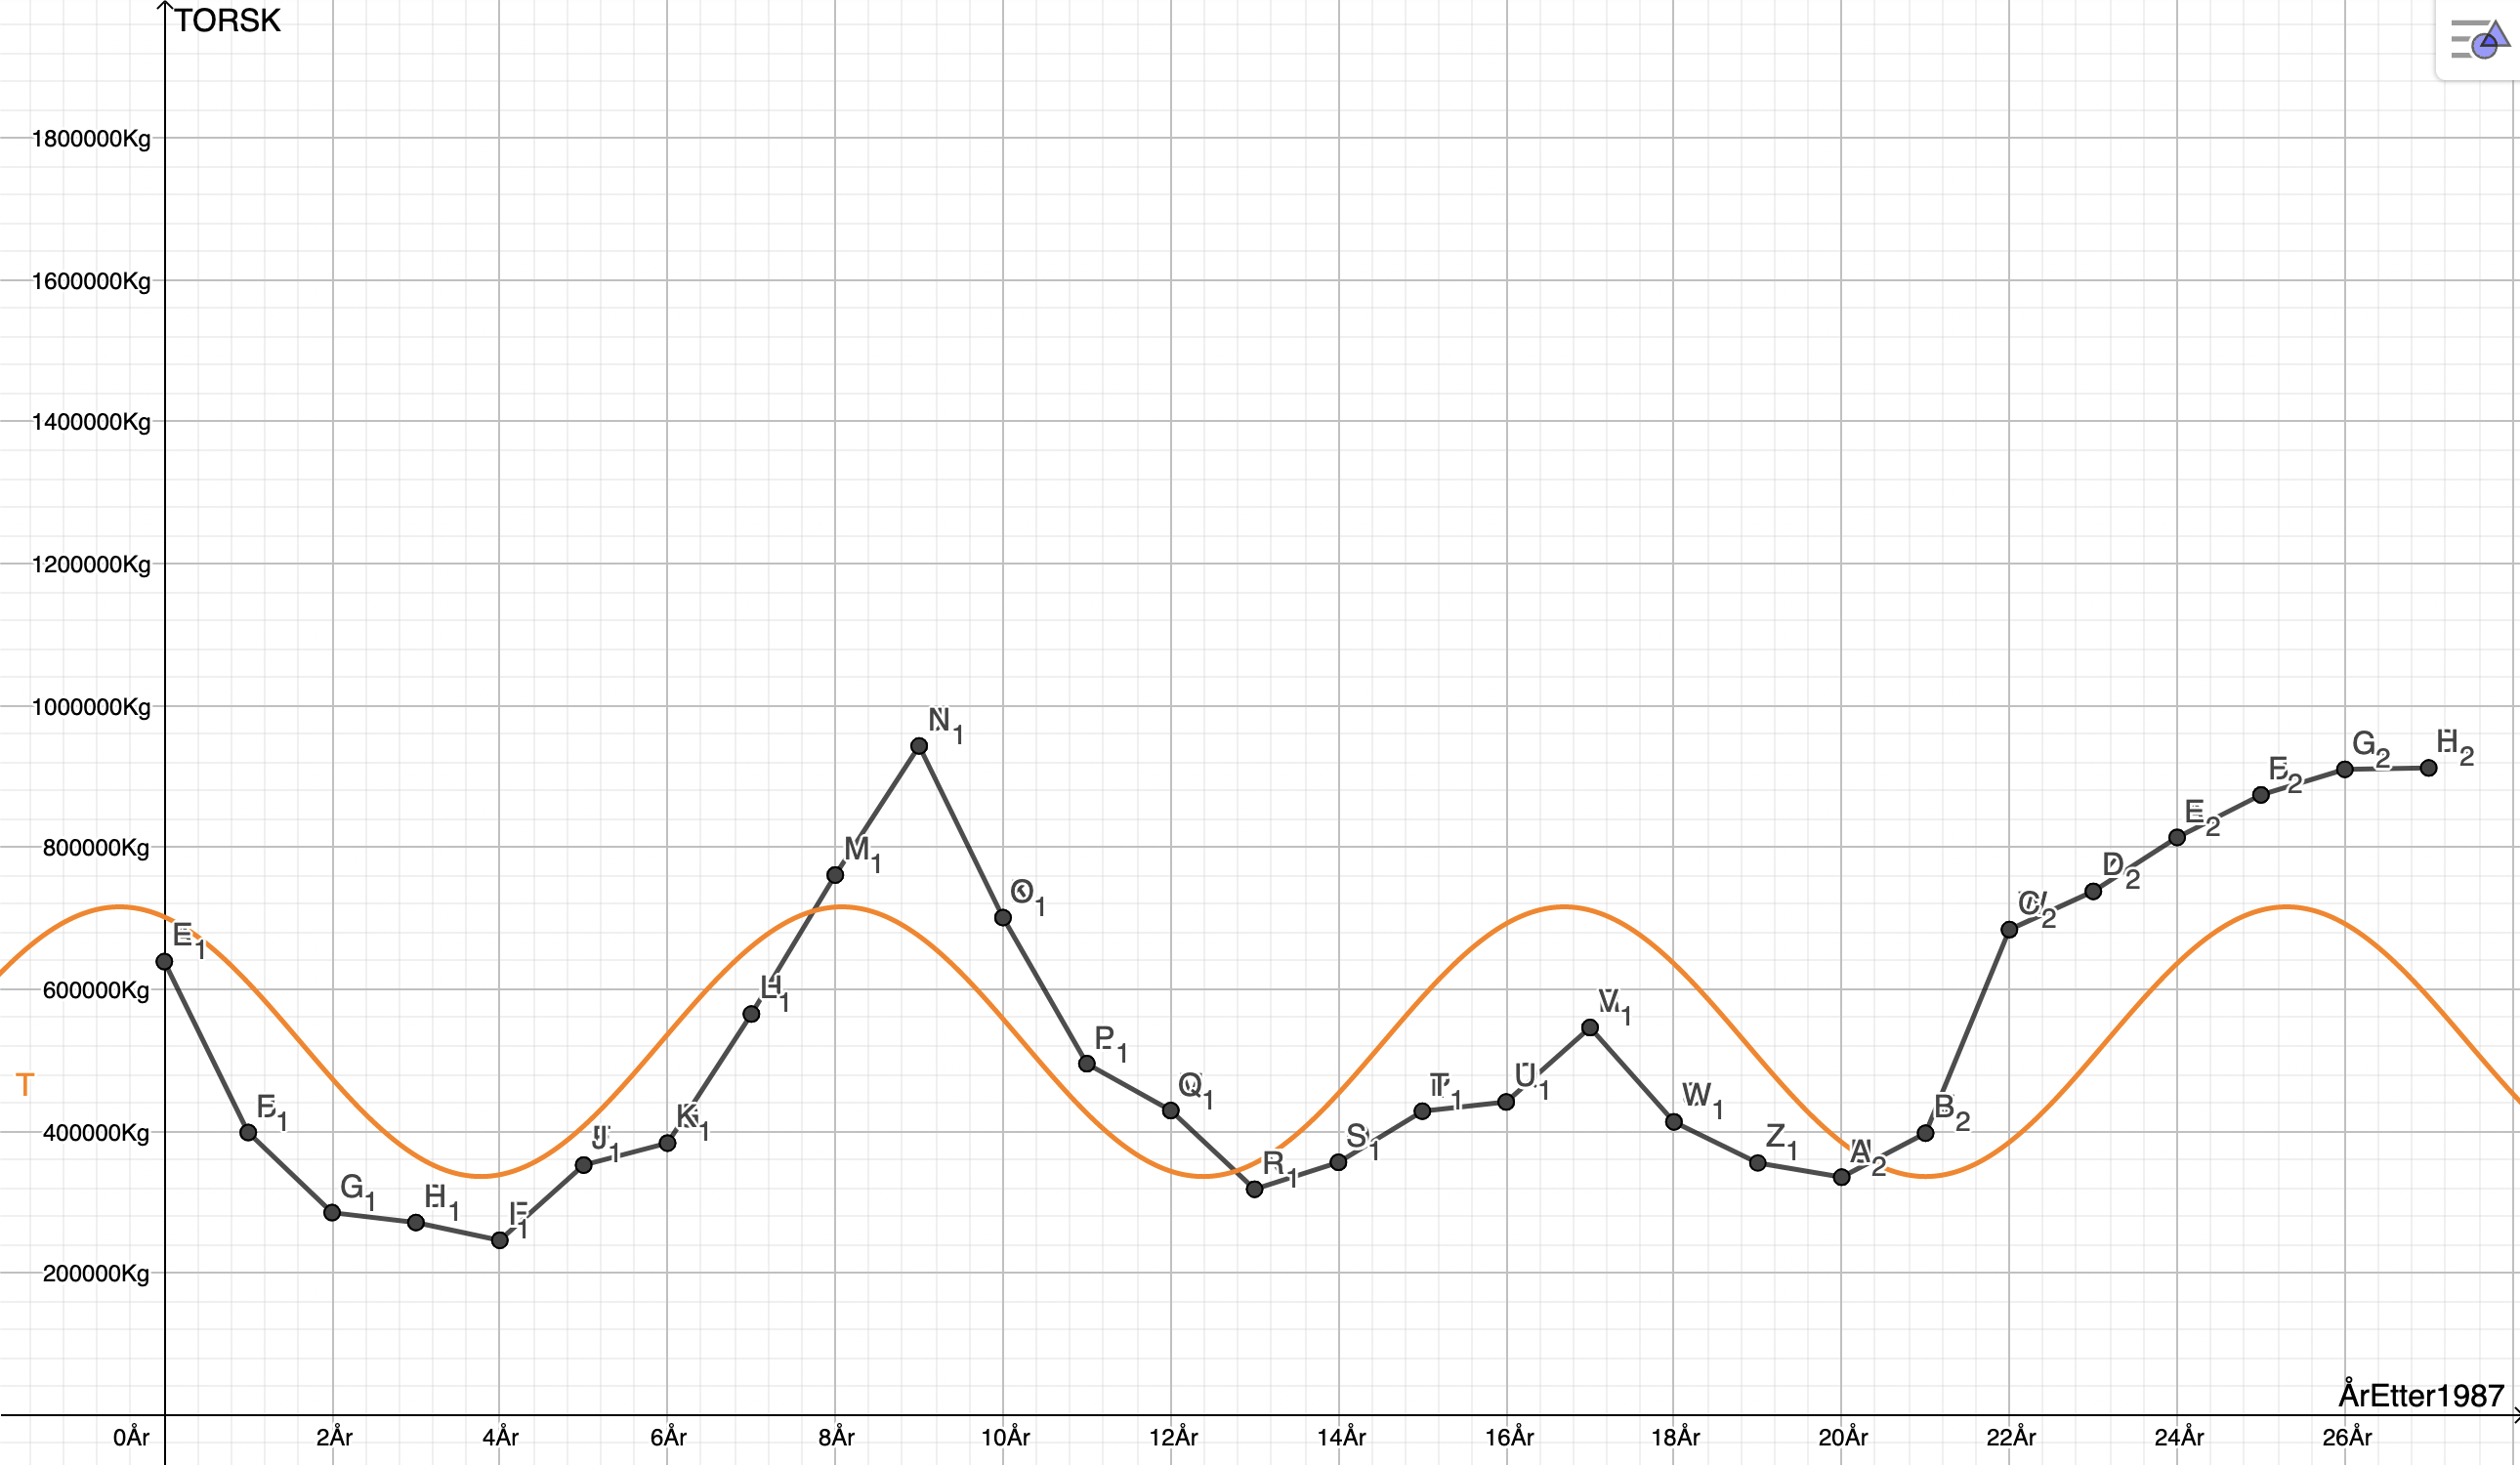
\includegraphics[scale=0.3]{Bileter/T.png}
	}
	\caption{Første regresjonsmodell $T(t)$}
	\label{T}
\end{figure}
Denne modellen tar omsyn til berre tidsperioden definert tidlegare (1987-2014), men ein anna modell som tar bruken av alt data og ikkje berre etter 1987 kan brukast.
Kva for ein modell som er meir presis og praktisk brukbar er diskuterbar, ettersom den sistnemnte har meir data kan den vere meir presis, men det er umogleg å vite om det oppstår nokon anomali ettersom dei andre faktorane manglar data som gjer at den kan vere meir upresis.
Denne sistnemnte modellen kan formulerast slik:
\begin{center}
	$T_{1}(t) = 393876+200559\times \sin(0.755t+1.45)tonn.$
	\textit{Her er t tall år etter 1987.}
\end{center}

\begin{figure}[H]
	\centering
	\fbox{
		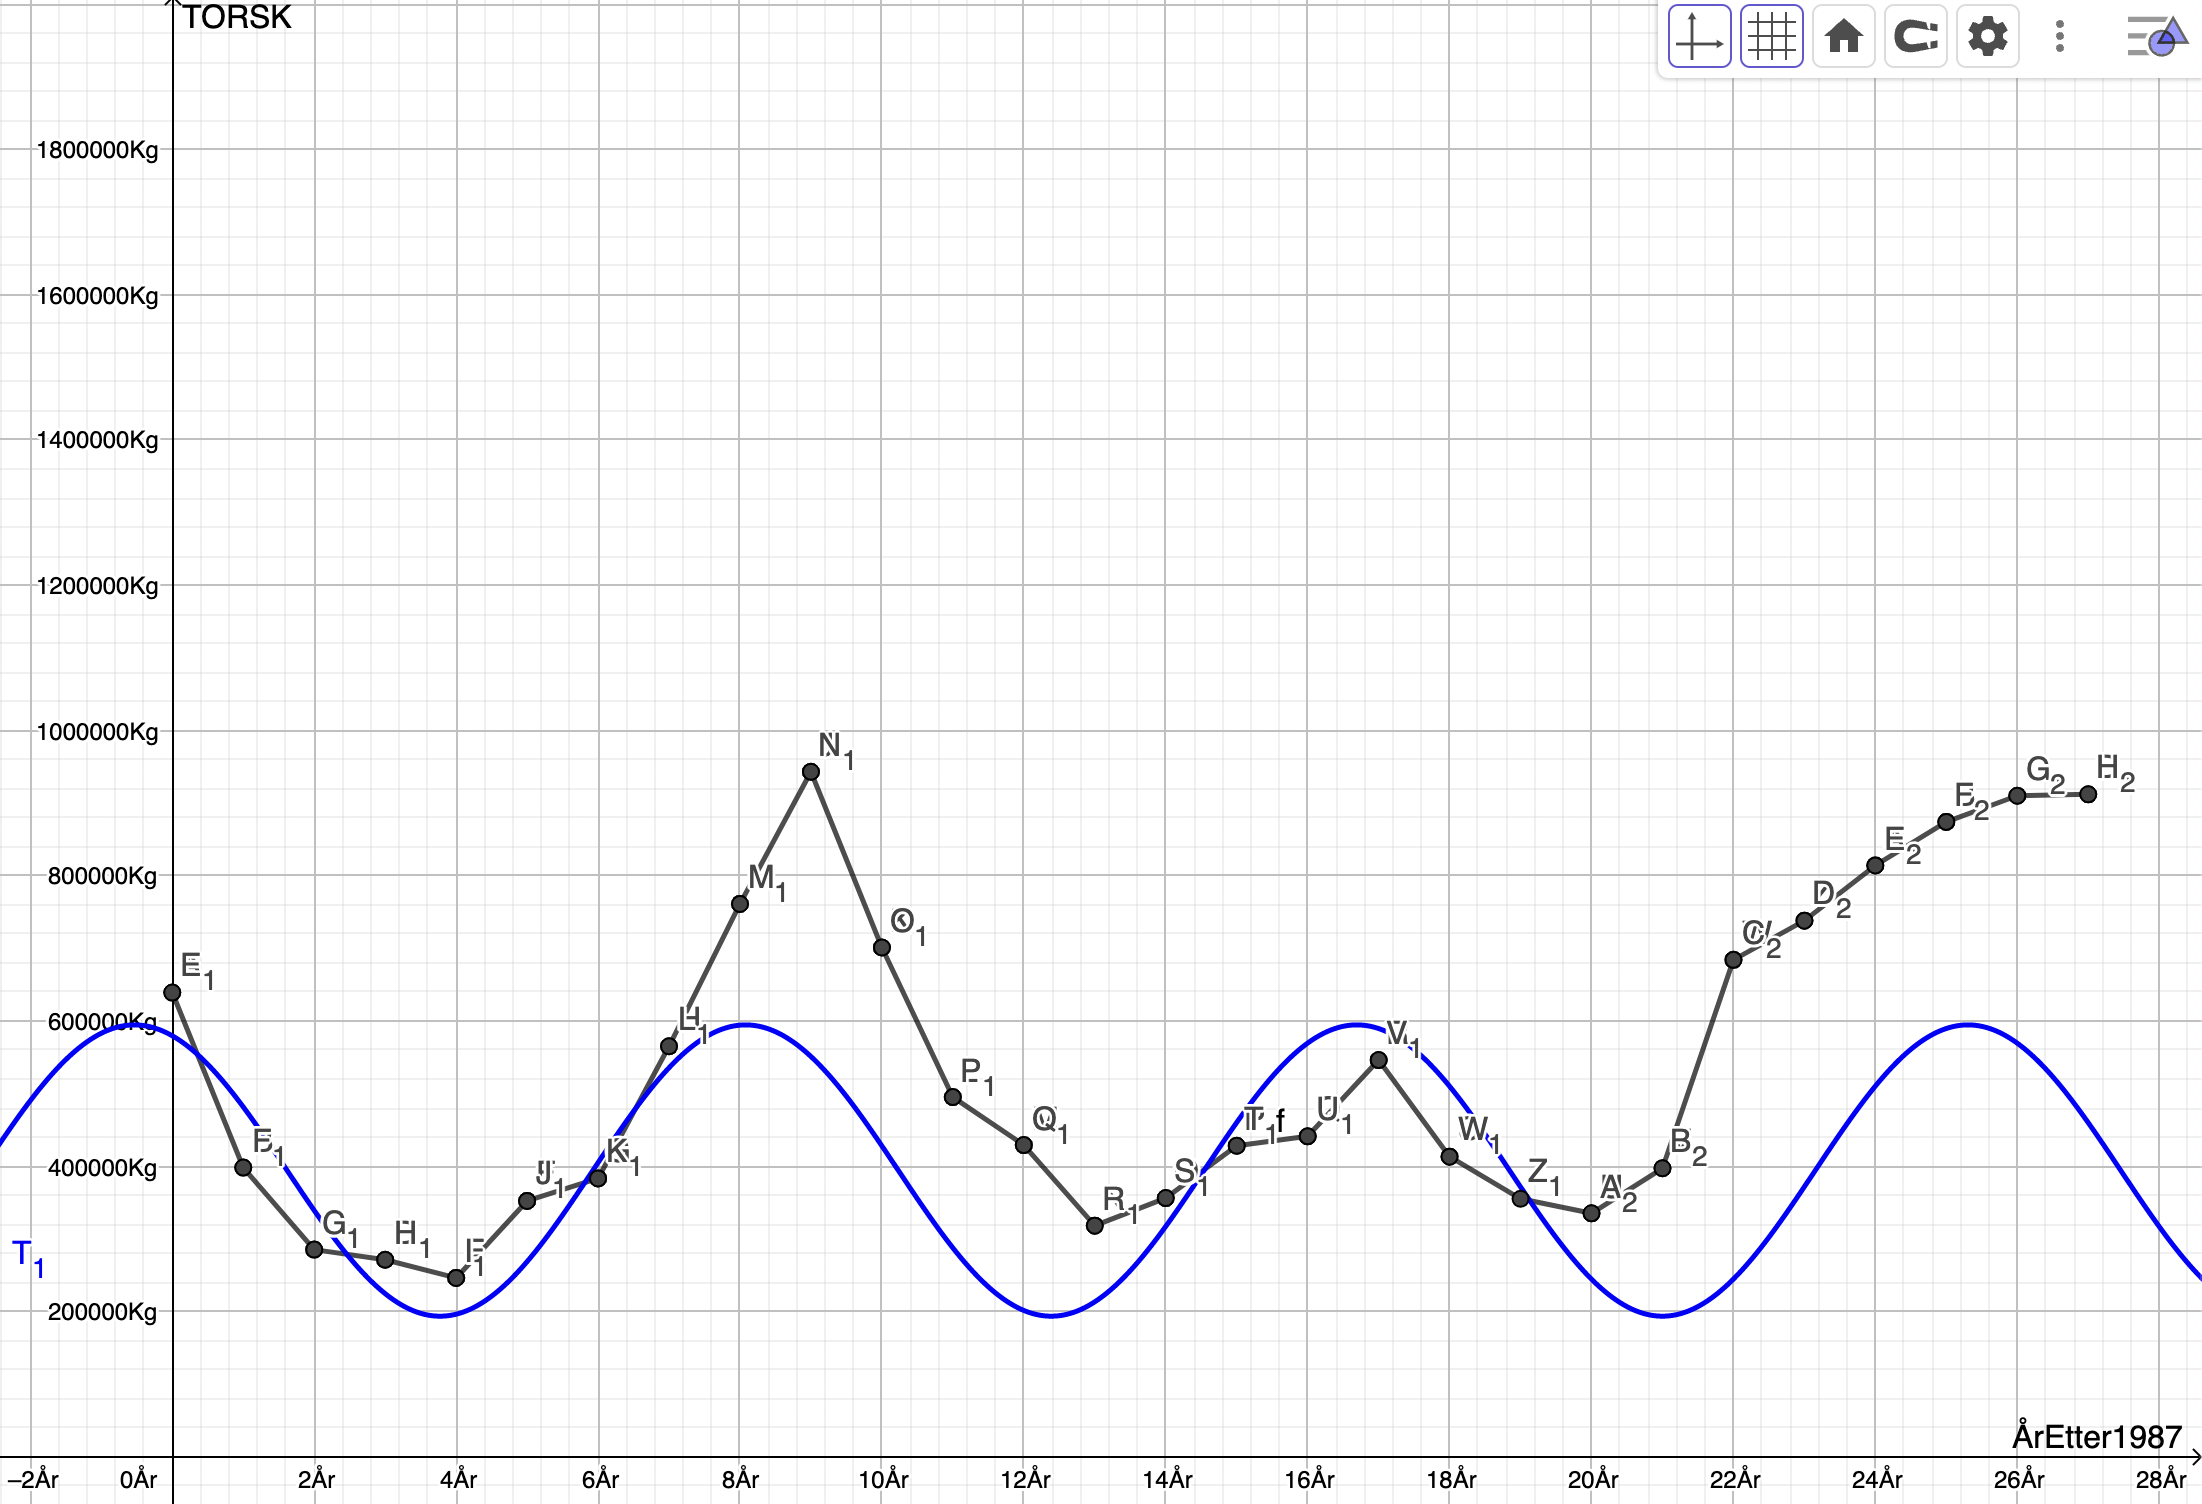
\includegraphics[scale=0.35]{Bileter/T1.png}
	}
	\caption{Andre regresjonsmodell $T_1(t)$}
	\label{T1}
\end{figure}

Modellar som berre nyttar årstal som inntaksverdiar for å rekna ut fiskebestand, kan ikkje betraktast som tilstrekkeleg nøyaktige. Desse modellane tek ikkje omsyn til utviklinga av andre faktorar som kan påverke bestanden. Vidare går desse modellane ut ifrå at det ikkje skjer noko utvikling over tid i fiskebestanden totalt sett, noko som ikkje alltid stemmer overeins med verkelegheita. I tillegg finst det andre farar og ulemper med desse modellane, sidan dei ikkje er i stand til å fange opp komplekse samspel mellom faktorar i havet, som til dømes temperatur og andre fiskebestandar.
Eit mogleg tilnærming for å ta omsyn til utvikling over tid og samspel mellom faktorar, er å kombinere ein lineær regresjon med ein sinusregresjon. Likevel er dette framleis ein usikker tilnærming som ikkje nødvendigvis viser samspellet mellom faktorar i havet, og kan derfor ikkje betraktast som ei fullverdig løysing.
Det er derfor behov for ein meir omfattande og sofistikert modell som kan ta omsyn til ei rekkje faktorar som kan påverke fiskebestanden. Ein slik modell vil krevje omfattande innsamling og analyse av data på tvers av ulike felt, inkludert økologi, biologi og meteorologi. Dette vil krevje samarbeid og samhandling mellom ulike forskingsfelt og sektorar. Ein slik modell vil imidlertid kunne gi ei meir helhetleg og nøyaktig forståing av korleis ulike faktorar påverkar fiskebestandane, og bidra til berekraftig forvaltning av desse ressursane.
Ein slik modell vil bli konstruert på slutten av rapporten.
\section{Veksten for fiskebestanden.}
Dersom ein ønskjer å undersøke når torskebestanden aukar eller minkar, kan ein nytte derivasjonsteknikkar for å utforske dette fenomenet.
Ved å derivere funksjonen som beskriv torskebestanden, vil ein kunne finne ut når den endrar seg positivt eller negativt.
Ein positiv derivert verdi vil indikere ei auking i torskebestanden, medan ein negativ verdi vil indikere ei minking. Vidare kan ein finne ekstremalpunkt ved å løysa for den deriverte sine nullverdiar. På denne måten er det mogleg å utforska og forstå endringar i torskebestanden og korleis den utviklar seg over tid.
Kunnskap om den deriverte kan vere svært nyttig for fiskeriindustrien i post-olje tida i Noreg. Ved å ha informasjon om endringar i torskebestanden, kan ein planlegge økonomisk for framtida. Identifisering av topp-punkter gjennom nullpunktane i den deriverte kan også gi praktiske tidspunkter for fiskeaktivitet, noko som kan føre til større og meir effektiv fangst. Dette kan ha positive effekter for både fiskeriindustrien og økosystemet i havet.
Det er verd å merka seg at derivasjon i seg sjølv ikkje gir ein fullstendig analyse av datamaterialet, men kan bidra til å finna interessante samanhengar og korrelasjonar.
For å få ei grundigare forståing av torskebestanden og dens utvikling, må ein ta i bruk ei rekke ulike analysemetodar og vurdera resultata av desse saman. Derivasjon er dermed ein verdifull tilnærming som kan bidra til å avdekka mønster og samanhengar i datamaterialet, og bør brukast som ein del av ei meir omfattande analyse.
\subsection{Derivasjon av regresjon.}
Ved å nytte tidlegare nemnde modellar for torskebestand er det mogleg å utvikle ei formel som kan rekne ut vekstfarten til torskbestanden i åra etter 1987 som input.
Modellane kan deriverast og dei deriverte funksjonane viser til den momentane vekstfarten (aukinga og minkinga) til torskebestanden.
Det er viktig å merke seg at dette berre gir ein omtrentleg verdi for vekstfarten.
Sjølv om det kan vise til vekstfarten til område utanfor det definerte tidsrommet, vil det ikkje vere heilt nøyaktig når det gjeld verkelegheita. Dette er fordi, som nemnd tidlegare, torskebestanden kan vekse på ein totalsettmåte, og modellen er berre ein omtrentleg estimasjon av bestanden.
Det er mogleg å utføre ein lineær regresjon for å finne ut om torskebestanden veks på ein totalt sett måte. Men det er ikkje sikkert om dette vil vere påliteleg i verkelegheita og kor lenge denne totale veksten sett vil vare, sidan datasettet er avgrensa.
Dermed ville dette ikkje halde påliteleg heller, og argumenterbart kanskje mindre truverdig. Ettersom den totale utviklinga av bestanden kan variere seg i sesongar også, og ein estimasjon som ikkje tar omsyn til totalsettutvikling vil dermed vere meir presis når ein grenseverdi-er tiden inn i det uendelege.
For å undersøkje vekstraten til modellen må ein ta i bruk matematiske derivasjonsreglar.
Ein kan derivere den første formellen gjennom å ta i bruk $kjerneregelen$, også kjent som $kjederegelen$ ($chainrule$ på eng.):
\begin{align*}
	T(t)  & = 526052+190105\times \sin(0.7295t+1.96)                \\
	      & = 190105 \times \sin(0.7295t+1.96)                      \\
	      & \textit{(Fjernar konstanten pga. eksponent regel.)}     \\
	      & = 190105 \times \sin(u), u=0.7295t+1.96                 \\
	      & = 190105 \times \cos(u) \times u'.                      \\
	      & \textit{(Deriverte av sin er cos, bruk kjerneregelen.)} \\
	      & = u' = 0.7295                                           \\
	      & = 190105 \times \cos(0.7295t+1.96)\times 0.7295         \\
	T'(t) & \approx 138682 \times \cos(0.7295t+1.96)
\end{align*}
\begin{figure}[H]
	\centering
	\fbox{
		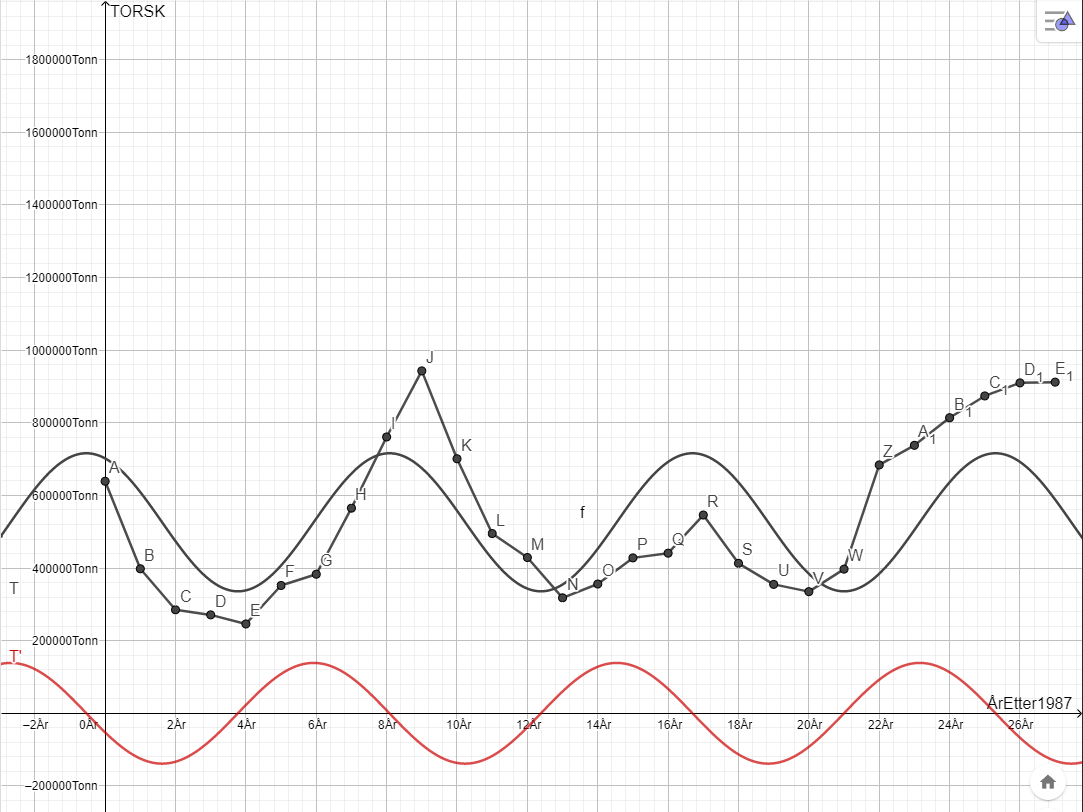
\includegraphics[scale=0.35]{Bileter/TDER.png}
	}
	\caption{Funksjon $T(t)$ (svart) og $T'(t)$ (raud) plottet i GeoGebra.}
	\label{TOGTDER}
\end{figure}
Ein kan gjere likt med den andre modellen for fiskebestanden som tar utgangspunkt i fleire datapunkter, men diskuterbart er meir usikker ettersom den tar ikkje omsyn til eventuelle anomali.
Den andre modellen sin deriverte er som følgande:
\begin{align*}
	T_{1}(t)  & = 393876+200559\times \sin(0.755t+1.45) \\
	          & ...                                     \\
	          & \textit{(Gjer likt som ved forrige.)}   \\
	          & ...                                     \\
	T_{1}'(t) & \approx 155433 \times \cos(0.755t+1.45)
\end{align*}
\begin{figure}[H]
	\centering
	\fbox{
		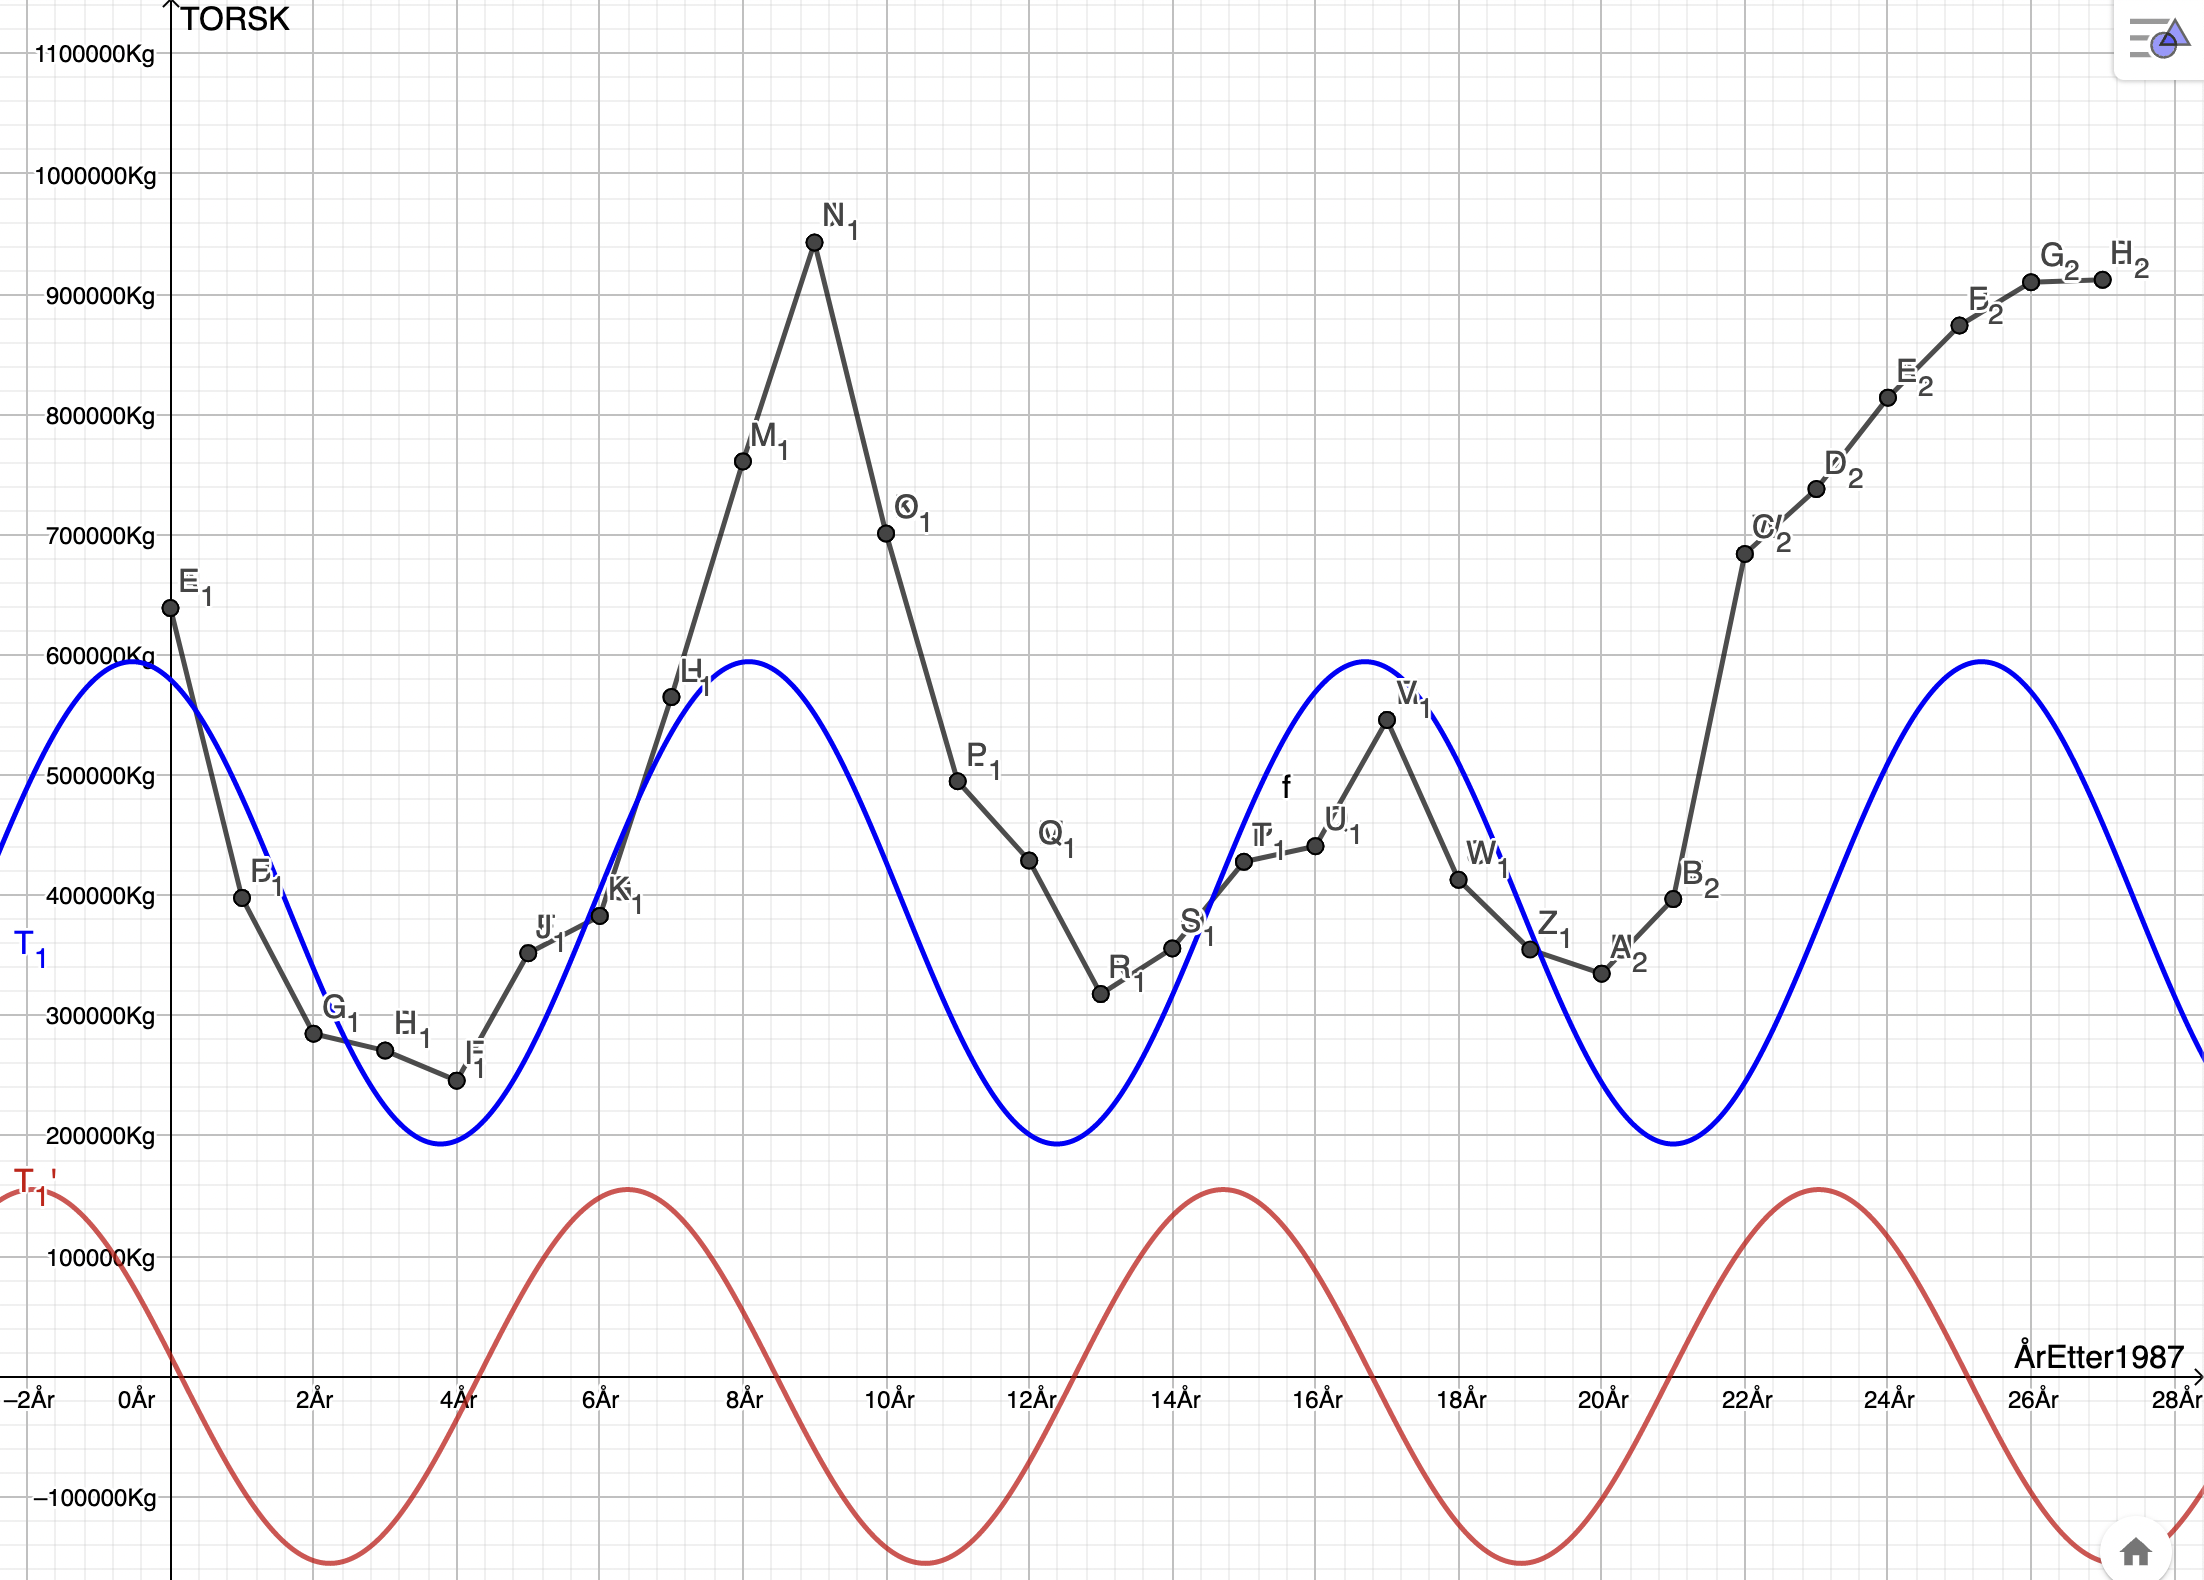
\includegraphics[scale=0.35]{Bileter/T1DER.png}
	}
	\caption{Funksjon $T_{1}(t)$ (blå) og $T_{1}'(t)$ (grønn) plottet i GeoGebra.}
	\label{F5}
\end{figure}
Frå herav vil berre den originale regresjonsfunksjonen $T(t)=526052+190105\times \sin(0.7295t+1.96)$ bli brukt ettersom den har ikkje moglegheita for anomali som oppstår i andre datasett der det ikkje er data tatt opp.
\subsubsection{Undersøke når fiskebestanden er på det høgaste/lågaste \& forandring i vekstrate.}
I mange situasjonar kan det vere av stor verdi å vite når torskebestanden når sitt høgaste og lågaste punkt. Dette gjeld ekstremt mykje for fiskeriindustrien, der kunnskap om når fiskebestanden er på sitt lågaste kan vere avgjerande for økonomisk planlegging.
I slike situasjonar kan det vere mindre gunstig å fiske, fordi fangstmengda kan vere lågare.
Omvendt kan kunnskap om når fiskebestanden når sitt høgdepunkt, gi gode moglegheitar for større fangster og dermed større økonomisk avkasting.
Identifisering av slike punkt kan dermed være en viktig faktor for fiskeriindustrien når det gjelder strategisk planlegging og økonomisk utbytte.
\begin{align*}
	T'(t) & = 190105 \times 0.7295 \times \cos(0.7295t+1.96)                                    \\
	      & 190105 \times \cos(0.7295t+1.96)\times 0.7295 =0                                    \\
	      & \textit{Dividerer på } 190105\times 0.7295                                          \\
	      & \cos(0.7295t+1.96) =0                                                               \\
	      & \textit{cos(a)=0, når } a=\pi n-\frac{\pi}{2}, \textit{der n er ein reell integer.} \\
	      & 0.7295t+1.96 = \pi n -\frac{\pi}{2}                                                 \\
	      & 0.7295t = \pi n - \frac{\pi}{2}-1.96                                                \\
	      & t = \frac{\pi n - \frac{\pi}{2}-1.96}{0.7295}
\end{align*}
Ved å undersøke dei to første $n$ verdiane av funksjonen som beskriv vekstbestanden når funksjonen når sitt høgaste og lågaste punkt, og derav også når veksten aukar eller minkar.
Dei første 3 løysingane for denne $t=\frac{\pi n - \frac{\pi}{2}-1.96}{0.7295}$ likninga er $n=0$, $t_0\approx -4.84$, $n=1$, $t_1\approx -0.534$, $n=2$, $t_2\approx 3.773$.
Her er det viktigt å merke seg at kvart $2n$ vil vere like høg i verdi hos $T(t)$ funksjonen, dette er sesongane sin topp og botnpunktar.
Ved å settje den første $t_0$ verdien inn i funksjonen $T(t_0)$ får ein $335947tonn$, ein verdi som lågare enn konstanten til $T(t)$: $526052$. Noko som tyder til at dette er eit botnpunkt.
Dette tyder også til at $t_1$ sin verdi er eit topppunkt, $T(t_1)$ får ein verdi av $716157tonn$.
Ut i frå dette tyder det til at kvart $t_{1+2n}$ er topppunkter og $t_{2n}$ er botnpunkter. Mellom topppunktene og botnpunktene vil det alltid skje ei minking i torskebestanden, og mellom botnpunktene og topppunktene vil det skje ei auking.
Ein kan også finne ut kor mykje tid som det går mellom kvart topppunkt og botnpunkt ved å finne differansen mellom to etterfølgjande $t_i$ verdier.
Tida det tar mellom kvart botnpunkt og topppunkt er då $|t_2 - t_1| \approx 4.3$år og mellom kvart topppunkt og det neste topppunkt, eller mellom kvart botnpunkt og det neste botnpunkt, er $|t_2-t_0| \approx 8.6$år.
\subsubsection{Finne ut når bestanden sin vekst snur seg.}
I fiskeriindustrien er det avgjerande å forstå utviklinga og tilstanden til fiskebestandane for å oppretthalde berekraftig fiskepraksis.
Ein effektiv måte å oppnå dette på er ved å bruke regresjonsmodellar som gir ein matematisk beskriving av bestandens vekst over tid.
Ved å ta den dobbeltderiverte av regresjonsmodellen kan ein avdekke informasjon om endringa i bestandens veksthastighet, og på den måten oppnå ein betre forståing av korleis bestanden utviklar seg over tid.
Vendepunktet i regresjonsmodellen indikerer når veksten endrar seg frå positiv til negativ eller omvendt.
Denne informasjonen er svært verdifull for fiskeriindustrien, sidan det kan indikere når det er på tide å intensivere overvaking og undersøking av bestanden, samt investere fleire ressursar i å ta vare på den.
Endringar i veksthastigheita kan vere forårsaka av miljøendringar, og dette kan ha ein betydeleg innverknad på havmiljøet.
Dersom det ikkje var ein akselerasjonen på bestanden, noko som er naturleg ekstremt vanskeleg å oppnå, kunne bestanden risikere enten fullstendig utrydding eller eksponentiell vekst, og dette kan føre til ein konstant ustabil likevekt i naturen.
Ved å dobbelderivere og så løyse for 0 kan ein finne ut når bestanden sin vekstrate snur seg.
\begin{align*}
	T'(t)  & = 190105 \times 0.7295 \times \cos(0.7295t+1.96)                      \\
	       & = 190105 \times 0.7295 \times \cos(u), u=0.7295t+1.96                 \\
	       & = 190105 \times 0.7295 \times -\sin(u) \times u'.                     \\
	       & \textit{(Deriverte av cos er -sin, bruk kjerneregelen.)}              \\
	       & = 190105\times 0.7295^{2}\times -sin(0.7295t+1.96)                    \\
	T''(t) & \approx -101168 \times sin(0.7295t+1.96)                              \\
	       & \textit{Dividerer på } -101168                                        \\
	       & sin(0.7295t+1.96) = 0                                                 \\
	       & \textit{sin(a)=0, når } a=\pi n, \textit{der n er ein reell integer.} \\
	       & 0.7295t+1.96 =\pi n                                                   \\
	       & Q.E.D                                                                 \\
	       & t= \frac{\pi n -1.96}{0.7295}                                         \\
\end{align*}
Dei tre første løysingane for likninga $t=\frac{\pi n -1.96}{0.7295}$ er $n=0$, $t\approx -2.69$, $n=1$, $t\approx 1.62$, $n=2$, $t\approx 5.93$. Desse verdiane er av betydning og kan vere særleg viktige. Å bruke denne likninga kan dermed vere av stor grad av betydning i fiskeriindustrien, og kan kome til nytte i verkelegheita, ettersom ho modellerer når vekstraten snur seg og fiskebestanden byrjar å vekse eller minke i vekst.
\subsection{Numerisk derivasjon av datasettet gjennom Python for bruk i framtidige studiar.}
Ein effektiv måte å derivere eit datasett er å bruke numerisk derivasjon, som er ei tilnærming basert på det opphavlege datasettet, her ved hjelp av Python.
Dette er spesielt nyttig når ein ønsker å analysere historiske data og når ein vil bruke resultatet av denne analysen i framtidige studiar av fiskebestanden i Barentshavet.
Fordi den skaffer den deriverte over berre datasettet og ikkje modellar.
Sjølv om denne metoden er praktisk og rask, kan den vere litt upraktisk i nokre situasjonar, ettersom den berre gir gjennomsnittlege vekstfart over året, og gir ikkje innsikt til vekstfarten i dei einskilde månadene.
Det bør òg nemnast at det siste datapunktet i datasettet ikkje kan derivere, sidan det manglar data for neste år. I samsvar med definisjonen av den gjennomsnittlege deriverte, $\frac{\Delta y}{\Delta x}=\frac{y_f-y_i}{x_f-x_i}$, kan dette ikkje reknast ut fordi det manglar data for både $y_f$ og $x_f$. Så sjølv om numerisk derivasjon kan vere ein nyttig teknikk, er det viktig å vere merksam på dens avgrensingar og å bruke den forsiktig.
\newline\newline
Den følgande Python-algoritme var skapt og tatt i bruk:
\begin{verbatim}
    import pandas as pd
    import matplotlib.pyplot as plt

    # Last inn data
    fil = "torsk.csv"
    datafil = pd.read_csv(fil, sep=",", comment="#", decimal=".")
    yakse = datafil["TORSK"].tolist()

    #Liste over modell data.
    xVerdier=[]
    yDerivertVerdier=[]

    #Teikne diagram over målte data.
    for i in range(len(yakse)):
        xVerdier.append(i)
        yakse[i]=yakse[i]*1000 #Frå '000 tonn til tonn.

    plt.plot(xVerdier,yakse,"x")


    #Modeller den deriverte.
    for x in range(len(yakse)-1):
        derivert = yakse[x+1]-yakse[x] #(yf-yi)/(xf-xi) xf-xi=1
        print(derivert)
        yDerivertVerdier.append(derivert)

    #Vis derivert saman med målte data.
    xVerdier.pop()
    plt.grid()
    plt.plot(xVerdier,yDerivertVerdier)
    plt.xlabel("År etter 1987.")
    plt.ylabel("Torskmengde.")
    plt.show()
\end{verbatim}

\begin{figure}[H]
	\centering
	\fbox{
		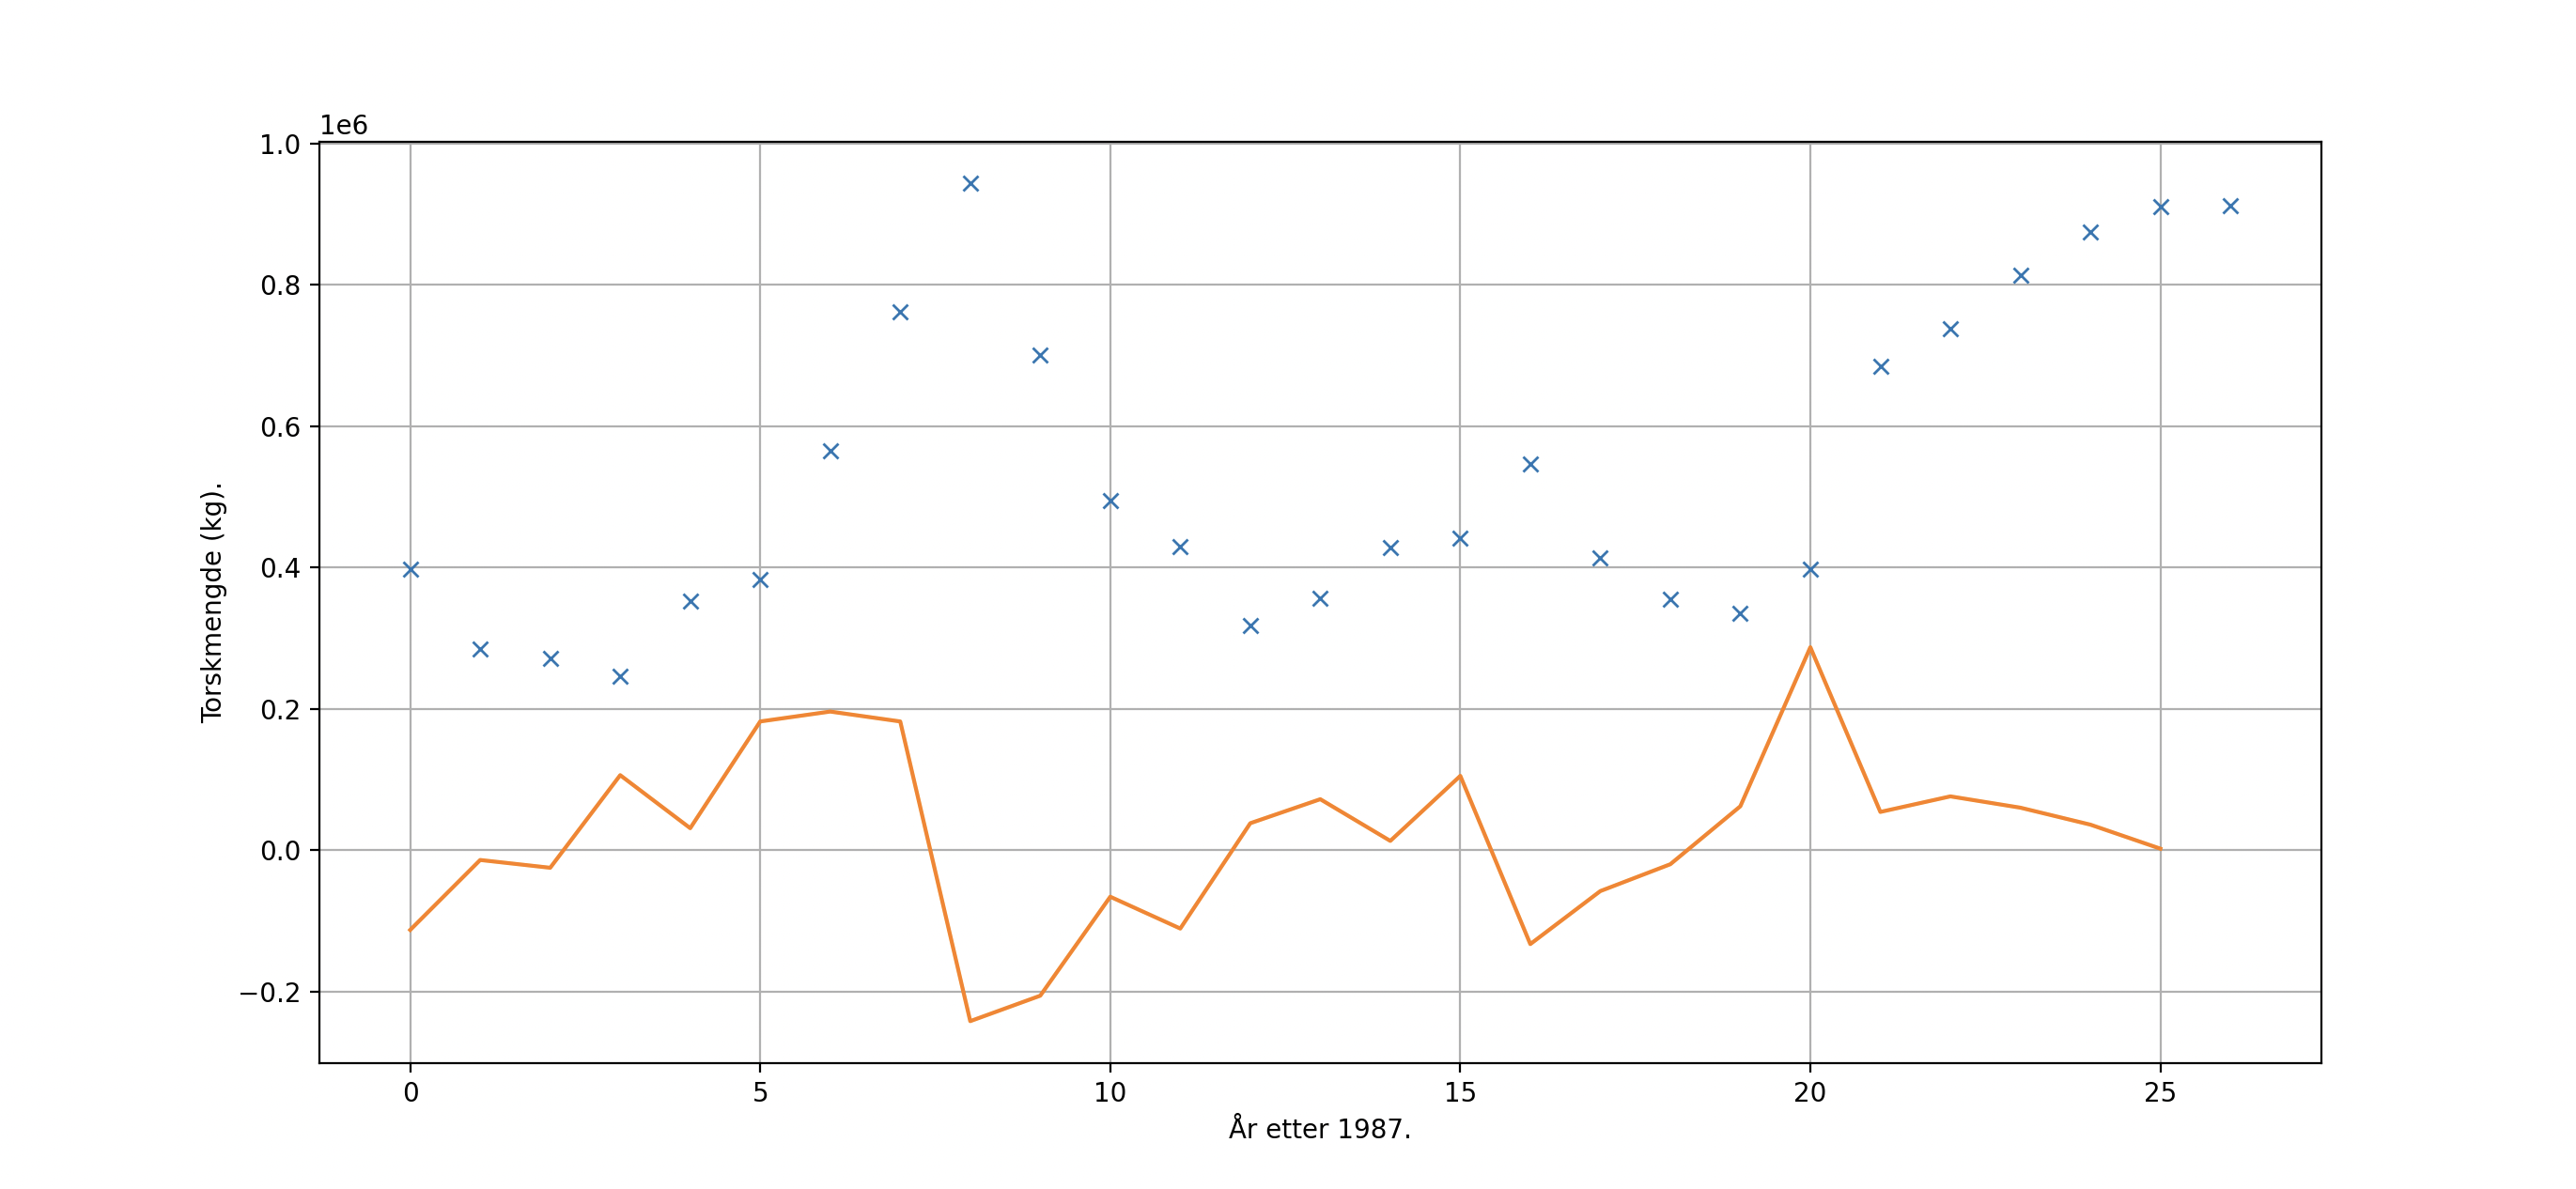
\includegraphics[scale=0.3]{Bileter/NumeriskDerivasjon.png}
	}
	\caption{Numerisk Derivasjon.}
	\label{F4}
\end{figure}

Den numeriske derivasjonen viser her endringa i verdien av torskebestanden over tid, og kan vere eit nyttig verktøy for å forstå fortidsdata og prediktere framtidige trendar i framtidige studiar av torskebestanden.
Ved å analysere grafen til funksjonen kan ein identifisere korleis nøyaktig dette datasettet utvikla seg utover tida. Dette gir ein meir presis analyse over datasettet, regresjonen sin derivasjon er berre ein god tilnærming. Til dømes kan ein seie at den numeriske derivasjonen er høgast rundt år 20, der grafen viser størst auking i verdien av grafen.
På same måte kan ein seie at den numeriske derivasjonen har lågast verdi rundt år 8, der minkar grafen mest.
Det som er merkbart er at det ikkje er ein fin utvikling i den deriverte utover tida, slik som oppstår ved regresjonen sin deriverte, dette indikerer mykje hos torskebestanden. Blant anna, at det kan vere mange påverkande faktorar med varierande frekvenser, som kan påverke bestanden.
Det viser også at regresjoner ikkje skaper ein heilt presis modell for røynda, røynda er ofte meir kaotisk og nyansert enn det matematikk kan modellere.
\section{Finne totalmengde torsk målt.}
For å berekne totalt tal torskefisk som har levd i Barentshavet over denne tidsrammen, nyttast ei metode som kallast integrasjon.
Integrasjon kan definerast som ei matematisk operasjon som gjer det mogleg å berekne arealet under ei kurve, og kan praktisk talt representere total fiskebestand målt over ei gitt tidsramme.
Å ha kunnskap om totalt tal torskefisk som har levd i Barentshavet vil vere av stor verdi for framtidige studiar og undersøkingar av dette datasettet, då det gir ein meir heilskapleg oversikt over bestanden.
Integrering kan utførast på fleire måtar, mellom anna ved numerisk berekning i programmeringsverktøyet Python, eller ved å nytte integrasjonsreglar i matematikk.
Matematisk kan ein definere ein ein integrasjon slik: $\int_{a}^{b}f(x)\delta x=\lim_{\Delta x \rightarrow 0^{+}}\sum_{n=a}^{\frac{b}{\Delta x}}f(n)$
\subsection{Å finne totalmengde torsk målt.}
Ein simpel numerisk integrering over datasettet gir den totalemengda av torsk som har blitt målt i havet over tidsrammen datasettet har.
Denne integreringen har ikkje upresise verdier og kan lett oppnås gjennom bruken av Python, dette kan også oppnås gjennom simpel matematikk, men fordi datasettet var lagret i $.csv$ format var dette enklast.
Python koden er identisk til den matematiske funskjonen av $\sum _{i=0} ^{27} (TorskMengde_{i})$, 27 år er tidsrammen sin totale lengde. Formelen tar alle verdier av målt torskemengde per år i tidsrammen og summerer dei saman.
\begin{verbatim}
    import pandas as pd

    # Last inn data
    fil = "torsk.csv"
    datafil = pd.read_csv(fil, sep=",", comment="#", decimal=".")
    codDataSet = datafil["TORSK"].tolist()
    #Finn total mengde torsk som har levd.
    total = 0
    for i in codDataSet:
        total+=float(i)*1000 #Må gjere over frå '000 tonn til tonn.
    print(f'Total mengde torsk målt er {total}tonn')
\end{verbatim}
Svaret er då at mengda torsk som har levd i fiskebestanden over dei 27 åra har hatt ein totalmasse som er rundt $14350000tonn$.
Ved å dele på 27, tall år, finner ein den gjennomsnittlege mengda torsk vekt målt per år i tidsrammen, $\frac{14350000tonn}{27}\approx 531481tonn \approx 530000tonn$.
Ein viktig og nyttig kunnskap er å vite kor mykje torsk som er i barentshavet, for å finne ut dette kan ein dele på $11/1000$, dette er fordi ein gjennomsnittleg atlantisk torsk som bur ut i havet har ein vekt på $11kg$ (Mass.gov), rapporten måler i tonn så det blir delt på $1000$ for å gjere det til tonn, dette er den presise gjennomsnittlege vekt.
Det er framleis viktig å merke seg at torsk har blitt observert til å kunne vere opptil 50 kilogram i vekt i sære spesielle tilfeller, og dette skaper ein viss usikkerheit i dataen.
Ein kan då analysere at den generelle torskebestaden per år er omtrent rundt $\frac{531481}{11/1000}\approx 48316454torsk \approx 48000000torsk$ i mengde.
Det er også mogleg å modellere den momentane bestanden i torsk gjennom å ta i bruk regresjonsmodellen og denne konstante vekt verdien.
Ein funksjon som gir torskemengda kan dermed modellerast slik $Torsk_{Mengde}(t)=\frac{T(t)}{11/1000} \rightarrow\frac{526052+190105\times \sin(0.7295t+1.96)}{11/1000}\rightarrow\frac{526052}{11/1000} + \frac{190105}{11/1000}\times \sin(0.7295t+1.96)\approx 47822909+17282272\times \sin(0.7295t+1.96)$.
I følgje modellen vil det vere omtrent $Torsk_{Mengde}(36)\approx 48726944 \approx 49000000$ torsker i Barentshavet i starten av 2023. Sjølvsagt vil dette avvike og variere utover året, indikert av den deriverte modellen drøftet fram tidlegare.
Vidare kan denne funksjonen utviklast til å ta inn ein sekundær variabel som forklarer konstanten, dette er nyttigt dersom det visast til at konstanten er upresis til røynda.
Denne andre funksjonen kan drøfast slik: $Torsk_{Mengde,1}(t,k)=\frac{T(t)}{k}\rightarrow \frac{526052+190105\times \sin(0.7295t+1.96)}{k}$. Der $k$ er eit reellt tall.
Som nemnt tidlegare, det er også svært viktig å merke seg at desse mengde-torsk modellane kan vere delvis upresis i verdi, ettersom den same fiska kan bli målt fleire gonger, vekten varierer frå kvar torsk og det er umogleg å vite nøyaktig kor mykje torsk det er, utan å vite kvar torsk sin vekt.
Men dette er diskuterbart framleis ein svært god estimasjon som kan vere praktisk nyttig.
\subsection{Å anslå presisjonen til den originale regresjonsbaserte modellen gjennom integrasjon.}
Ved å bruke dei tidlegare nemnde modellane for torskebestanden over tid, kan ein prøve å nytte integrasjonsreglar for å rekne ut den totale torskebestanden som har vorte fiska opp i målinnretningane.
Det er likevel viktig å merke seg at denne integrasjonsmodellen kan vere unøyaktig over datasettet i dette tilfellet, sidan regresjonen er ein tilnærming til datasettet som gjeld den bestemte tidsperioden.
Likevel kan det seiast at denne modellen kan nyttast over større tidsperiodar enn berre datasettet og kan dermed ha praktisk nytte i framtidige studiar også.
Det er viktig å vere merksam på desse avgrensingane når ein nytter seg av modellen og å ta omsyn til eventuelle feilkjelder, som utvikling av torskebestanden totaltsett, som kan påverke resultata.
Ein kan då utføre integrasjonen slik:
\begin{align*}
	T(t)              & = 526052+190105\times \sin(0.7295t+1.96)                                  \\
	                  & = 526052t+190105\times\sin(0.7295t+1.96)+c_{1}                            \\
	                  & = 526052t-190105\times\frac{\cos(0.7295t+1.96)}{0.7295}+c_{1}             \\
	\int T(t)\delta t & =526052t-190105\times\frac{\cos(0.7295t+1.96)}{0.7295}+c_{1}              \\
	                  & \textit{(Frå eit praktisk perspektiv vil $C_1$ vere 0 i verdi i røynda. )} \\
					  & \textit{(Vi skal berre summere, ingen ekstra konstant $C_1$.)} \\
	TotalT(t)         & =526052t-190105\times\frac{\cos(0.7295t+1.96)}{0.7295}
\end{align*}
For å finne kor mykje torsk som har blitt målt, i følge den regresjonsbaserte modell intregasjonen, må ein definere området vi skal finne arealet under grafen til, her er det frå 0 til 27 ettersom det er 27 år med data:
\begin{align*}
	\int_{0}^{27}T(t) \delta t & = [TotalT(t)]_{0}^{27} \\
	                           & = TotalT(27)-TotalT(0) \\
	                           & \approx 14449543-98884 \\
	                           & \approx 14350659tonn
\end{align*}
Denne verdien er særleg nær den numeriske intregrasjonen med eit avvik på berre $14350659tonn-14350000tonn=659tonn$, noko som tyder til at denne regresjonsmodellen kan halde godt på å estimere den totale målte bestanden over fleire tidsrammer.
Dette låge avviket på berre $659tonn$ viser ekstremt godt kor presis denne modellen er når det kjem til integrasjon og å forsøke å finne ut kor mykje torsk som er i havet i ein tidsperiode.
Det er framleis viktig å nemne at torskebestanden kan variere og utvikle seg på metodar og vegar som modellen ikkje tar omsyn til, dette gjer at denne integrasjonsmodellen framleis halder seg litt upresis når det kjem til større tidsområder enn det som var definert tidlegare.
Framleis er dette ein indikator til modellen kan halde presis, og dermed kan den diskuterbart vere god og praktisk brukbar.
Ut i frå dette oppstår det viktige spørsmålet om kor presis denne tidsbaserte modellen er til røynda, det hadde vore svært nyttefullt å vite kor mykje avviket frå modellen er til røynda på gjennomsnitt.
\section{Å finne den gjennomsnittlege avviket frå røynda.}
MAE (Mean Absolute Error), eller "Middelavvik", er ein måte å måle feil mellom modellprediksjonar og faktiske verdiar i eit datasett.
Det er definert som gjennomsnittet av absoluttverdiane av differansen mellom prediksjonane og dei faktiske verdiane.
I andre ord så er det den gjennomsnittlege forskjellen i verdi frå røynda og modellert verdi, det er det gjennomsnittlege avviket.
Formelt sett kan dette uttrykkjast som $MAE = \frac{1}{n}\times \sum_{i=0}^{n}(|y_i - \hat{y_i}|)$, der $y$ er modellens prediksjonar, $\hat{y}$ er dei faktiske verdiane, og $n$ er talet på datapunkt i datasettet.
MAE kan brukast som ein måte å evaluere kor godt ein modell kan estimere faktiske verdiar i verkelegheita.
I dette tilfellet blir MAE brukt til å finne ut kor presis vår tidlegare oppgitte tidsbaserte modell er i forhald til røynda og dens observerte data.
Å vite kva MAE-et er kan hjelpe fiskeindustrien med å forutsjå kor mykje upresisheit det er i mengda torsk dei kan fange i eit gitt år, og planlegge deretter.
Det bør imidlertid merkast at MAE er avhengig av at modellen ikkje har ein auking absolutt sett, noko som ein ikkje kan vite med den korte datamengda observert, den 27 år lange tidsramma skapar også ein liten usikkerheit i å vite kor presis denne målinga på upresisheit haldar seg.
Derfor kan estimata som er basert på MAE, vere litt upresise og bør tolkast med forsiktighet.
For å utrekne kva denne MAE verdien er kan ein dessverre ikkje ta i bruk det matematiske programmet \textit{GeoGebra} og det var dermed naud for å bruke ein anna metode for å rekne ut dette.
Her blei det brukt \textit{Python} for å gjere dette raskt, effektiv og presist.
\begin{verbatim}
    import pandas as pd
    import math

    # Last inn data
    fil = "torsk.csv"
    datafil = pd.read_csv(fil, sep=",", comment="#", decimal=".")
    codDataSet = datafil["TORSK"].tolist()

    #T(t) = 526052 + 190105 × sin(0.7295t + 1.96), årstall etter 1987.
    def regresjonsModel(årstall):
        return 526052+190105*math.sin(0.7295*årstall+1.96)

    #Kalkuler MAE, MAE = 1/n × Sum i=0 => n (|y_i − y_iˆ |).
    def kalkulerMAE():
        midlertidigVerdi = 0
        for i in range(len(codDataSet)):
            regresjonsVerdi = regresjonsModel(i)
            ekteVerdi = float(codDataSet[i])*1000 #Over frå '000 tonn til tonn.
            midlertidigVerdi+=abs(ekteVerdi-regresjonsVerdi)
        return midlertidigVerdi/len(codDataSet)


    MAE = kalkulerMAE()
    print(f'MAE er {MAE} i verdi.')
\end{verbatim}
Gjennomsnittleg absolutt feil (MAE) har vist seg å vere ein relativt låg verdi av $\approx 156019$tonn som gjengiven av \textit{Python}-koden, sjølv om ho framleis er noko høg. Dette indikerer at det er avgjerande å vere forsiktig med modellen sidan ho ikkje har ein merkbar låg MAE.
Likevel kan MAE brukast til mange føremål i denne konteksten og forklarar korleis grafen ser ut og kor presis ein må vere i diskusjonen av modellen.
Det bør imidlertid nemnast at MAE ikkje refererer til den maksimale skilnaden modellen kan ha frå verkelegheita, noko som teknisk sett er umogleg å forutsjå sidan datasettet kan utvikle seg annleis og nye maksimale skilnader kan oppstå.
Likevel er MAE ein god indikator på at modellen er nøyaktig i mange tilfelle, og gjer henne til ei god og påliteleg modell, basert på datasettets avgrensa perspektiv på den potensielle totale utviklinga av torskebestanden i Barentshavet.
Dette er òg ei indikasjon på at for å oppnå ein perfekt modell, som nøyaktig modellerer verkelegheita med ekstrem presisjon, må ein oppnå ein lågare MAE. Det er imidlertid ikkje mogleg å skape meir presise modellar med slike matematiske regresjonsmodellar som blir brukt her, for ein slik perfekt modell må ta omsyn til mange fleire faktorar, noko som kan tyde på at ei perfekt modell er umogleg å oppnå sidan data for tusenvis av faktorar ikkje er tilgjengelege på dette tidspunktet i historia.
Likevel er dette framleis ei ganske god og presis modell som kan brukast til mange praktiske føremål, og denne låge MAE-en beviser det. Denne modellen kan brukast i mange situasjonar, særleg i fiskeriindustrien der ho kan inkorporerast for å nøyaktig modellere forventa maksimale fangstmengder.

\section{Ein modell som tar omsyn til miljøfaktorar og andre fiskebestander.}
Ein multivariabel funksjon er ein matematisk funksjon som inneheld fleire uavhengige variablar. I motsetning til ein enkeltvariabel funksjon, der det berre er ein variabel som påverkar funksjonsverdien, kan multivariable funksjonar ha fleire variablar som påverkar resultatet. Dette kan vere nyttig i situasjonar der det er fleire faktorar som kan påverke eit resultat, slik som i økonomiske eller naturvitskaplege studiar.
I denne samanhengen blei det forsøkt å lage ein multivariabel funksjon for å analysere samanhengen mellom ulike faktorar og miljøfaktorar i høve til torskebestand.
I eit forsøk på å lage ein multivariabel funksjon på forma $y=bx_1 +b_2x_2 +b_3x_3 +b_4x_4+b_5x_5+c$, vart Excel si multivariable regresjonsmodell nytta.
Denne modellen viser samanhengen mellom dei ulike faktorane og miljøfaktorane, i tillegg til tid, men det er framleis viktig å merke seg at denne modellen er delvis upresis.
Upresisheten kan forklarast gjennom manglande datamengde, og at det er mange fleire faktorar som kan påverke torskebestanden.
Desse faktorane er ikkje dei einaste som vil ha innverknad på torskebestanden, men dei er eit godt utgangspunkt for å analysere samanhengar. Det er forventa at det vil vere upresisheit med slike modellar som har manglande datamengde, noko som er påført av manglande offisielle undersøkingar og data rundt dette. Dette er likevel ikkje ein negativ ting, men nærare eit krav innanfor slike studiar som brukar nye data.
Som nemnt tidlegare, og observert i plottinga av datasetta, var ei auking i loddebestanden ansvarleg for at ei auking i torskebestanden skjedde i kort tid etterpå, ikkje momentant og samstundes.
Loddebestanden må først auke før torsken kan spise den auka loddebestanden. Denne logikken gjeld også dei andre faktorane, til dømes effeketen til temperaturen på torskebestanden vil skje i etterkant av temperaturendringa, kor raskt varierar frå faktor til faktor.
Dette indikerer til at faktorane har ein tilknyting til torskebestanden sin vekstfart og ikkje direkte til bestanden. 
Gjennom ein regresjon som tek inn dei andre faktorane sin deriverte som påverkar bestanden, og torskebestanden sin deriverte kan ein deretter bruke integrasjon til å finne ein modell som tek inn fleire faktorar og gir tilbake torskebestanden sin totale vekt.
Det er viktig å ta i bruk inntaksverdiane sine deriverte og ikkje deira ekte verdiar, fordi torskebestanden blir påverka av forandringa i dei andre faktorane, når loddebestanden minkar, aukar torskebestnaden.
For å ha derivasjons-data som modellen skal tilpasse seg til var den tidlegare numeriske derivasjonsmodellen tatt i bruk.
Ved å ta i bruk tidlegare oppgitt oppsett kan ein omformulere den til å passe med torskebestanden: \newline
På forma $Torsk'_{2}(Lodde,Salt,Temp$\textit{År)}$=\beta_1$\textit{År}$ +\beta_2 Temp+ \beta_3 Salt + \beta_4 Plankton+\beta_5 Lodde$.
Her er det viktig å merka seg at lodde målast i $tonn$, salinitet i $\frac{kg}{m^2}$, temperatur i $celsius$ og tid i \textit{år} etter 1987.
I frå Excel får ein koeffisientene til $\beta_i$, $\beta_1$ er $0$, $\beta_2$ er $-0.473$, $\beta_3$ er $507818620$, $\beta_4$ er $9255000$, $\beta_5$ er $-7.444E-03$.
Då blir modellen til torskebestanden sin deriverte slik:
\begin{center}
	$T'_{2}(Lodde,Salt,Temp,$\textit{År)}$ \approx 0*$\textit{År}$ -0.473*Temp + 507818620*Salt + 9255000*Plankton - 7.444*10^{-3}*Lodde$
\end{center}
Det er viktig å vere kritisk til desse koeffisientene, og ikkje leggje dei som solid grunnlag for alle analyser.
Når koeffsientene er negativ betyr dette at dei har ein positiv påverknad i torskebestanden, ein negativ koeffisient multiplisert med ein negativ derivant hos ein faktor vil lede til eit positiv-derivant-ledd hos torskebestanden.
Når dette integrerast vil dette framleis halde presis, ein høg loddebestand vil ha ein låg torskebestand og omvendt.
Ved å integrere denne modellen for torskebestanden sin derivasjon finner ein torskebestanden sin totale tonn vekt, formulert gjennom faktorar som påverkar bestanden.

\begin{center}
	$T'_{2}(Lodde,Salt,Temp,$\textit{År)}$ \approx 0*$\textit{År}$-0.473*Temp + 507818620*Salt + 9255000*Plankton - 7.444*10^{-3}*Lodde $\\
	$\approx \frac{-0.473}{2}*Temp^2 + \frac{507818620}{2}*Salt^2 + \frac{9255000}{2}*Plankton^2  -\frac{7.444}{2}*10^{-3}*Lodde^2 + C_1$\\
	$\approx -0.237*Temp^2 + 253909310*Salt^2 + 4627500*Plankton^2 -3.722*10^{-3}*Lodde + C_1$\\
	\textit{Her vil det berre modellerast sesongane og ikkje bestanden.}\\
	\textit{Ved å settje C-konstanten til gjennomsnittet av bestanden er modellen meir presis.}\\
	$T_{2}(Temp,Salt,Plankton,Lodde) \approx -0.237*Temp^2 + 253909310*Salt^2 + 4627500*Plankton^2 -3.722*10^{-3}*Lodde^2 + 531481$
\end{center}

\begin{figure}[H]
	\centering
	\fbox{
		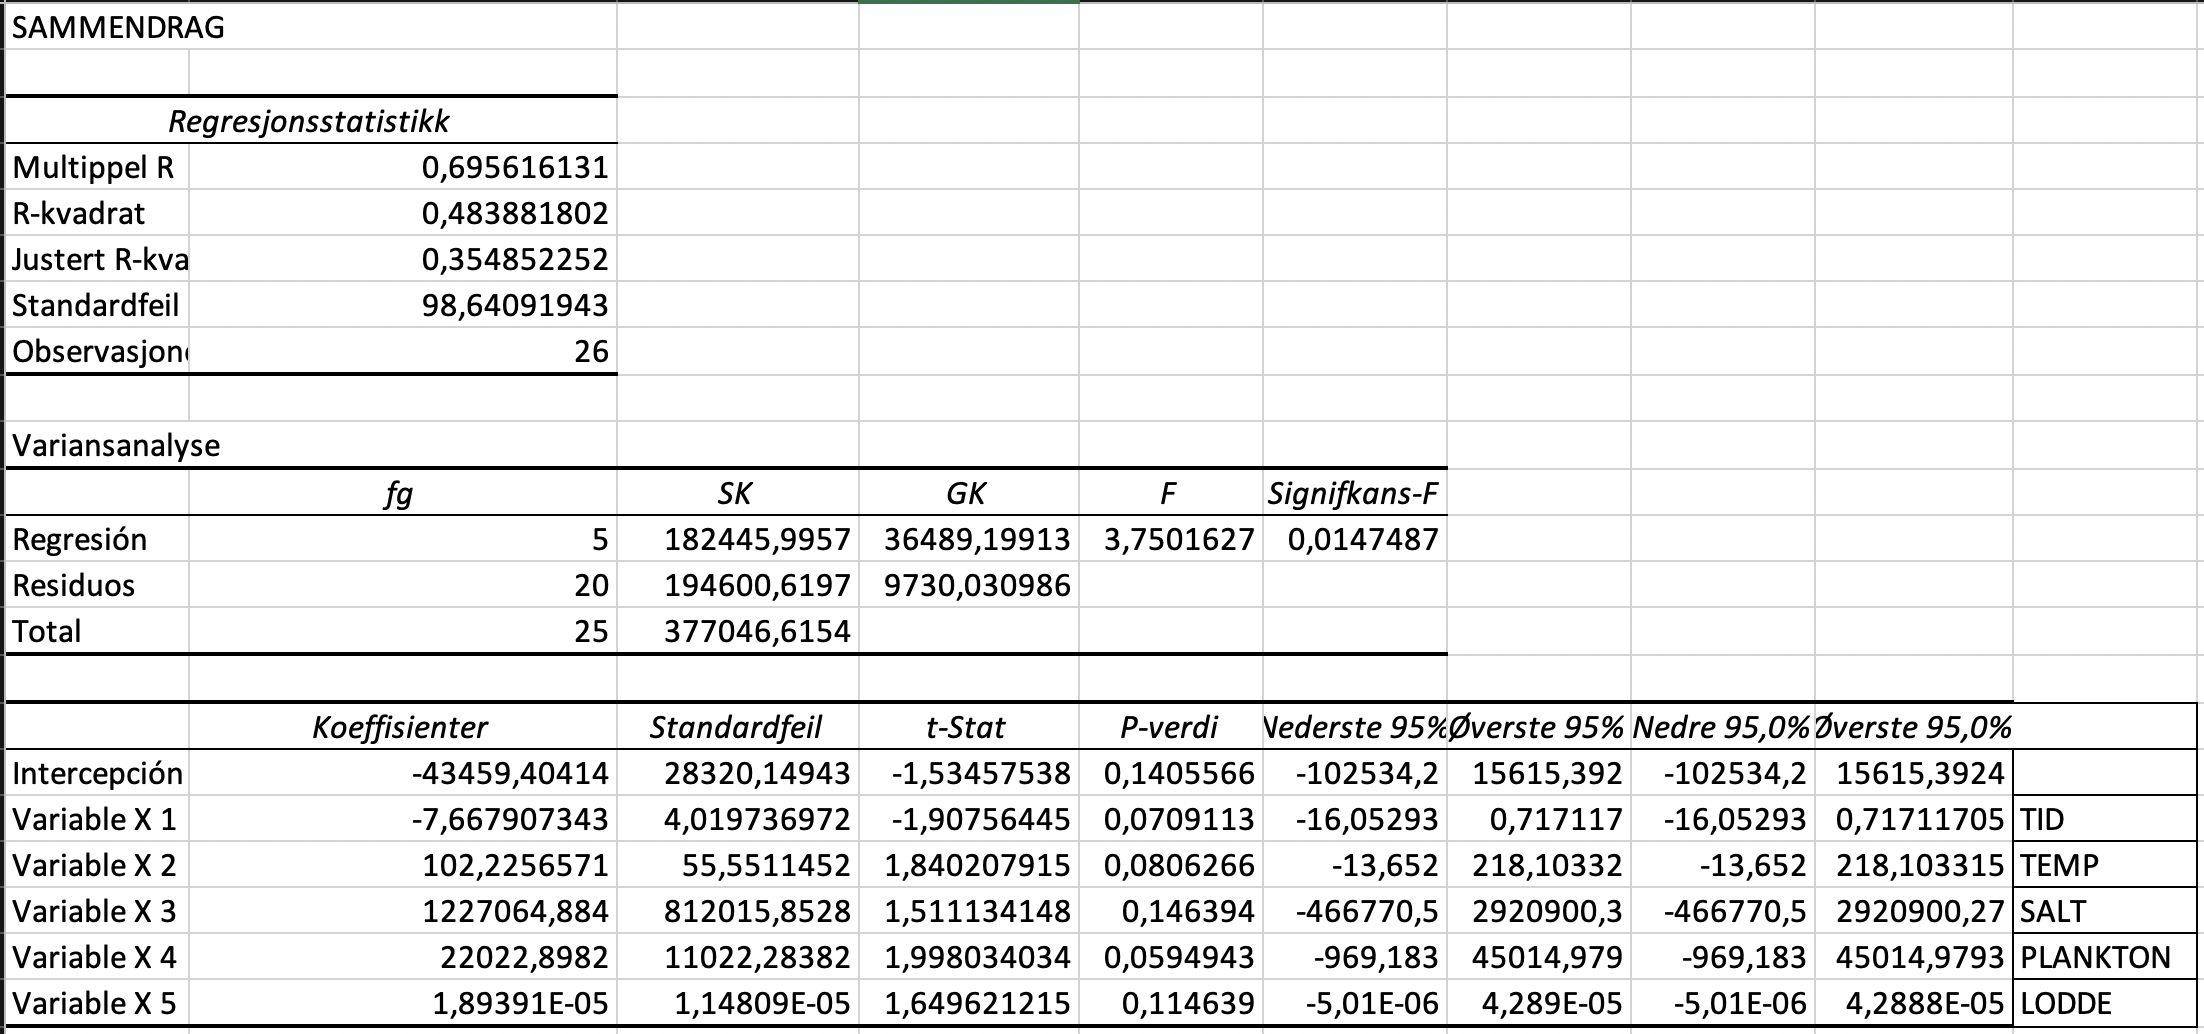
\includegraphics[scale=0.39]{Bileter/MultiVariabel.png}
	}
	\caption{Multivariabel regresjon resultater i frå Excel.}
	\label{Multi}
\end{figure}
Den multivariable regresjonsmodellen indikerer ein stor samanheng mellom loddebestanden og torskebestanden. Ein høg loddebestand fører til auka torskebestand, og dette blir indikert av den negative koeffisienten, og kan tydeleg bli observert i dei tidlegare plottet grafane.
Sjølv om denne koeffisienten er relativt låg i samanlikning med nokre andre koeffisientar som plankton, er loddebestanden likevel ekstremt betydningsfull på grunn av dei høge verdiene den har i inntaksverdi. Inntaksverdiane til lodde er svært høge noko som skaper eit ledd i funksjonen som er svært påverkande til resultatet av funksjonen.
Tid er ein faktor som ikkje viser nokon effekt på torskebestanden som heilskap. Dette gir sjølvsagt meining, sidan bestanden ikkje har nokon klar forståing av kva tid er og ei torsk klarer ikkje å tilpasse livsstilen sin etter mengda år etter 1987.
Likevel er det viktig å ta omsyn til tid då det kan indikere ein påverknad av menneskeleg aktivitet. Ein positiv eller negativ koeffisient til tiden ville innebere at det var ein tidsavhengig variabel, som menneskeleg aktivitet som har spesifikke tidsrammer, men dette er ikkje avklart til å være presist her.
Det er difor framleis svært viktig å sjekke slike moglegheiter i starten av denne multivariable analysen.
Salinitet har ein stor påverknad på torskebestanden, sidan torsk er ein saltvatnfisk som krev salt for å kunne trivast.
Ein altfor høg salinitet derimot vil ha ein negativ effekt på torskebestanden, for mykje salt vil settje det indre miljøet til torsken i ubalanse, noko som vil lede til større sjanse for daud.
Dermed er også koeffisienten til salinitet positiv. Temperatur har ein låg verknad på bestanden, der ein god varmare temperatur har ein positiv effekt på torskebestanden, men i liten grad. Den har dermed også ein negativ koeffisient, noko som tyder på at torsken kan like ein god temperatur.
Likevel er dette ikkje heilt presist sidan ein altfor stor temperatur, som $100C^o$, vil vere skadeleg for fisken i verkelegheita, noko som var nemnt i teori-biten, for mykje varme kan lede til oksygenmangel.
Plankton har ein negativ effekt på bestanden. At koeffisienten til plankton er positiv er ein litt uventa indikajson på at torsk har mange ulike rovdyr som spis den, ei auking i plankton indikerer ei auking i rovdyr noko som i resultat vil lede til ei minking i torskebestnaden.
Framleis er det viktig å anerkjenne at plankton er også viktig for torskebestanden i røynda, ein plankton mengde av $0$ ville ha skapt ingen næringsinntak til næringskjeden, noko som tyder til at den ville ha vore ein faktor som minkar bestanden totaltsett.  
Den multivariable regresjonsmodellen kan gje viktige innsikter i samanhengen mellom ulike faktorar og torskebestanden.
Likevel er det viktig å vere varsam med koeffisientane og modellen som heilheit, særleg når datasettet er relativt lite og kompleksiteten høg.
Koeffisientane kan vere feilaktige på grunn av manglande data eller unøyaktigheiter i modelleringa.
På trass av dette kan modellen fungere som eit godt utgangspunkt for å undersøkje samanhengane mellom ulike faktorar og torskebestanden.
Det er likevel viktig å påpeike at denne modellen ikkje fangar opp alle faktorane som kan påverke torskebestanden, det er ein svært høg kompleksitet rundt dyrebestander.
Framtidige, meir sofistikerte modellar vil kunne ta i bruk fleire datapunkt og faktorar for å gi eit meir presist bilete av denne komplekse samanhengen.
Denne modellen kan framleis, likevel den kan bere med seg upresisheitar, vere ekstremt nyttefull for fiskeriindustrien når det kjem til fangst av denne fiskebestanden. 
\chapter{Feilkjelder.}
Ved analysen av torskebestanden i Barentshavet er det viktig å vera merksam på ulike mogelege feilkjelder som kan påverke resultatet. Ein av dei mest opplagte feilkjeldene kan vere mangelen på data, spesielt i denne kort tidsrammen av berre 27 år. Dette kan til dømes skuldast teknologiske avgrensingar i innsamling av data eller utilstrekkeleg ressursallokering for å samle inn data på ein jamnleg basis. Mangelen på data kan føre til at nokre av parameterane i modellen ikkje er like nøyaktige som dei kunne ha vore om meir data var tilgjengeleg.
Ein annan potensiell feilkjelde kan vere feil i dei matematiske utrekningane og modellane som blir brukt. Sjølv om slike feil er sjeldne, er det framleis ein mogelegheit, særleg om modellane er kompliserte og datamaskinane som blir brukt for utrekningane, ikkje er optimalt programmert eller konfigurert. Ein måte å minimere slike feil på, er å bruke fleire uavhengige metodar for å modellere dataa og deretter samanlikne resultatet frå ulike modellar.
Ein annan mogeleg feilkjelde er at modellen ikkje tek omsyn til utviklinga av torskebestanden totalt sett. Til dømes kan endringar i klima og miljøforhold påverke torskebestanden på måtar som modellen ikkje kan føreseie. Dette kan føre til at modellen undervurderer eller overvurderer bestanden i enkelte situasjonar. Det er viktig å vera merksam på desse faktorane og å justere modellane og analysane etter behov.
Andre potensielle feilkjelder kan inkludere menneskelege faktorar som påverkar datainnsamling og analyse. Dette kan omfatte bias i datainnsamling eller utveljing av data som påverkar resultatet. Det kan også vere feil i berekningar eller tolkingar av resultatet. Det er viktig å vera kritisk til metodane som blir brukt i analysane, og å validere resultatet med fleire uavhengige kjelder.
Til slutt er det generelt viktig å vera kritisk til dei fleste studiane ein les, og å vurdere resultatet basert på kvalitet og relevans av dataa, validitet av analysane og rimelighet av konklusjonane. Forsking er ein kontinuerleg prosess, og det er alltid mogelegheit for forbetring og justering av modellane og analysane i lys av nye data og kunnskap.
\chapter{Konklusjon.}
Torskebestanden i Barentshavet er ein viktig og verdifull ressurs for fiskeriindustrien i Noreg, spesielt med tanke på den økonomiske betydninga etter oljealderen. Ein matematisk forståing av korleis bestanden utviklar seg og er samanhengande med andre faktorar, når den er på topp og når den er på sitt lågaste, er difor viktig for å optimalisere fiskeriaktivitetar og bevare bestanden på lang sikt.
Ein tidsbasert sinusforma modell blei utvikla for å analysere og modellere bestanden, med ein undersøking av endringar i bestanden og dens vekstfart ved hjelp av derivasjonsteknikkar.
Formelen for denne tidsbaserte sinusforma modellen var som følgande: $T(t) = 526052+190105\times \sin(0.7295t+1.96)tonn$.
Ekstremalpunkt og vendepunkt i modellen blei rekna ut og kan henholdsvis gi verdifull informasjon til fiskeriindustrien om når ein bør fiske eller ikkje, og når ein bør overvake bestanden meir eller mindre.
Ekstremalpunkta kan givast gjennom formelen: $t=\frac{\pi n - \frac{\pi}{2}-1.96}{0.7295}$, der $n$ er eit reellt tall og $t$ er tall år etter 1987. 
Kvar $2n$ vil vere lik i verdi etterfølgjande av at fiskebestanden går i sesongar.
Kvar $t_{1+2n}$ er eit topppunkt med verdi på $716157tonn$, kvar $t_{2n}$ er eit botnpunkt og har ein verdi på $335947tonn$.
Vendepunkta kan givast gjennom formelen: $t=\frac{\pi n -1.96}{0.7295}$, der $n$ er eit reellt tall og $t$ er tall år etter 1987.
Ein integrasjonsbasert utrekning blei også utført for å rekne ut storleiken på bestanden i gjennomsnitt per år, som viste seg å vere omtrent rundt $530000tonn$ eller $4800000 torsk$, basert på ein vekt på gjennomsnittlege $11kg$ per torsk.
Momentane modellar blei også utvikla ved å dele den tidsbaserte modellen på verdien $11kg$, ein slik modell var til dømes: $T_{Mengde}(t)=47822909+17282272\times \sin(0.7295t+1.96)$, der $t$ er tall år etter 1987.
Den tidsbaserte sinusforma modellen viste seg å vere svært presis med eit relativt lågt middelavvik (MAE) på omlag $156000kg$, noko som indikerer at den kan vere nyttig i praktisk bruk i fiskeriindustrien. Imidlertid må ein merke seg på at ein må også forvente at fangsten kan variere frå det forventa.
Ein modell som tek omsyn til fleire variablar kan vere enda meir presis og ta omsyn til unormale hendingar og andre uventa faktorar som den enkle tidsbaserte modellen ikkje kan. Excel si regresjonsfunksjon blei brukt til å utvikle ein slik modell, med numerisk deriverte verdiar av variablane og torskebestanden sine numeriske deriverte verdiar, og deretter til slutt integrere funksjonen.
Den resulterande modellen, som var $T_{2}(Temp,Salt,Plankton,Lodde) \approx -0.237*Temp^2 + 253909310*Salt^2 + 4627500*Plankton^2 -3.722*10^{-3}*Lodde^2 + 531481$, viste seg å vere nokså presis og kunne modellere fiskebestanden over tid med omsyn til nokre av dei viktigaste faktorane som påverkar bestanden.
Denne modellen kan vere ein viktig ressurs for fiskeriindustrien når det gjeld optimalisering av fiskeriaktivitetar og bevaring av bestanden på lang sikt.
Alt i alt, var mange ulike aspekt av bestanden utforska som kan vere praktisk brukbar, samlande skaper dette ein stor oversikt og forståelse over korleis denne fiskebestanden utviklar og oppførar seg. 
Fiskebestanden går i sesongar, som vist av den deriverte og den dobbeltderiverte, er påverka av ulike faktorar i miljøet, som lodde og temperatur, og modellane som drøftar den er samlasett ganske presise, som vist gjennom middelavviket og integrasjonen. 
\chapter{Forbetringar \& Ynsker \& Refleksjon}
Det finst fleire ulike metodar som kunne ha vorte brukt for å betre denne studien av torskebestanden. Ein betre planlegging av rapporten og ei grundigare undersøking av datasettet kunne ha gitt ei meir utfyllande rapport og ei meir nyansert forståing av datasettet. Ved å gjennomføre ei meir inngåande undersøking av naturen og livsstilen til torsken i Barentshavet, kunne ein ha oppnådd ein mykje større innsikt i mogelege faktorar som påverkar bestanden, og dermed også datasettet. Dette kunne ha gitt betre modellar og ei djupare forståing av torskebestanden sin utvikling.
Ved å nytte ein meir heilskapleg tilnærming og inkludere fleire ulike variablar, kunne det ha blitt identifisert potensielle truslar mot bestanden og føreslått tiltak for å oppretthalde ei berekraftig torskebestand i Barentshavet.
Viss det hadde vore gitt meir tid til prosjektet, ville eg ha ynskt å utforske fleire aspekt ved torskebestanden. Særleg ville eg ha likt å undersøke korleis andre faktorar og endringar i miljøet kan påverke torskebestanden over tid, og sjå nærare på samanhengane mellom desse faktorane for å analysere korleis ein kan drive ein berekraftig forvalting av torskebestanden og andre fiskebestandar utan å redusere torskefisket. Det ville også vore interessant å sjå på korleis datasettet utviklar seg som heilskap, og om det er mogleg å ta omsyn til dette når ein skapar modellar for torskebestanden. Det er viktig å påpeike at det ikkje nødvendigvis skjer ein total utvikling i datasettet i løpet av den tida det vart samla inn, og at denne utviklinga ikkje nødvendigvis indikerer ein total utvikling over ein lengre tidsperiode.
Vidare ville eg òg ynskt å undersøke korleis torskebestanden kan påverke andre fiskebestandar enn berre lodde. Sjølv om lodde blir antatt å være eit byttedyr for torsken, indikert av datasettet og den multivariable modellen, kan det også vera fleire fiskebestandar som lever i samspel med torsken. Til slutt ville det vore spennande å undersøke meir generelle matematiske modellar, som Lotka-Volterra differensiallikningar, som modellerer korleis bestanden utviklar seg mellom ulike rovdyr- og bytte bestander, og andre interessante modellar for bestanden. Ein breiare tilnærming til analysen av torskebestanden kan gi verdifull innsikt og betre grunnlag for å utvikle ein berekraftig forvalting.
Sjølv om det var nokre forbetringar som kunne vore gjort i studien av torskebestanden, som skrive om i tidlegare avsnitt, finn eg at den var godt gjennomført og effektivt utarbeidd. Eg var relativt effektiv både i planlegginga og utføringa av studien. Vidare var eg effektiv i skrivinga av rapporten, og eg klarte å skrive ein omfattande tekst som ga svært god innsikt i ulike aspekt ved undersøkinga. Dette omfatta ei diskusjon av upresisjonar i modellane, den praktiske nytten av modellane og undersøkingane som vart utført, og korleis matematikken som vart brukt var relevant og nyttig for å undersøke datasettet. Eg utførte òg matematikk som låg utanfor pensum og var avansert i innhald. Dette inkluderte å utforske nye, vanskelege matematiske tema som derivasjon av trigonometriske funksjonar, og multivariable funksjonar for å skape meir heilskaplege modellar som tek omsyn til ulike faktorar som påverkar torskebestanden. Eg brukte også integrasjon av trigonometriske funksjonar for å estimere bestanden av torsk og den totale mengda tonn målt. Python vart brukt til modellering og undersøking av datasettet. Til slutt nytta eg kjente statistiske måleiningar for å undersøke feil og unøyaktigheiter i modellane. Alt i alt er eg svært nøgd med denne rapporten, og eg ser fram til å utforske liknande biologiske og matematiske tema i framtida.
\chapter{Bibliografi.}
Wikipedia, (07.Mars.2023) \textit{Atlantic Cod}. Henta 15.03.2023 i frå: \\
\url{https://en.wikipedia.org/wiki/Atlantic_cod} \\ \\
Mass.gov, \textit{Learn more about atlantic cod}. Henta 16.03.2023 i frå: \\
\url{https://www.mass.gov/service-details/learn-about-atlantic-cod#} \\ \\
Havforskningsinstituttet, \textit{SJOMIL}. Henta 14.03.2023 i frå: \\
\url{https://www.imr.no/sjomil/} \\ \\
Wikipedia, (12.Feb.2023) \textit{Ecosystems}. Henta 14.03.2023 i frå: \\
\url{https://en.wikipedia.org/wiki/Ecosystem} \\ \\
\end{document}